% se puede agregar la opción [english] para 
%  memorias o tesis en inglés (borrando el archivo .aux)
\documentclass{umemoria} 

\depto{Departamento de Ciencias de la Computación}
\author{Alonso Utreras Miranda}
\title{IGACSE: Un videojuego educativo para enseñar algoritmos relacionados a grafos a estudiantes de Ciencias de la Computación}

% incluir ambos comandos para una doble titulación
%  o quitar el comando que no aplica
\memoria{Ingeniero Civil en Computación}
\tesis{Magíster en Ciencias, mención Computación}
%\tesis{Doctor en ???} % incluir solo este comando para doctorados

% puede haber varios profesores guía seperados por coma;
% pero si es una memoria, solo puede haber un profesor guía
\guia{Iván Sipirán Mendoza} 

% puede haber varios profesores co-guía seperados por coma;
% pero si es una memoria, el profesor co-guía será el primer
% integrante de la comisión
%\coguia{Nombre Completo Co-Guía} % incluir en caso de co-guía de *tesis*

%\cotutela{Nombre Institución} % incluir en caso de cotutela
% TODO: Agregar comision
% \comision{Nombre Completo Uno,Nombre Completo Dos,Nombre Completo Tres}

%\auspicio{Nombre Institución} % incluir en caso de recibir financiamiento

% tiene que ser el año en que se da el examen de título/grado (defensa)
%\anho{2021} % incluir solo para reemplazar el año actual

\begin{document}

\frontmatter
\maketitle

\begin{resumen}
% citas \cite{meegaplus}, pero no excelente \cite{MeegaPlusManual}
Los videojuegos educativos son reconocidos como herramientas motivadoras para enseñar y entretener a los estudiantes. Con el fin de validar estas afirmaciones, se han desarrollado diversos marcos de trabajo y se han realizado revisiones de literatura analizando el estado de arte y criticando cómo se realizan los estudios relacionados a videojuegos educativos. En este proyecto, se presenta IGACSE, un videojuego educativo diseñado para enseñar conceptos de grafos y los algoritmos BFS y DFS. Se utilizó la metodología MEEGA+  para evaluar la calidad de la aplicación, solicitando a dos grupos que probaran el juego y respondieran cuestionarios donde se le pregunta a los participantes por su percepción respecto del juego. El primero (N=15) realizó una prueba académica después de contestar el formulario. Este grupo, sin conocimiento previo de grafos, obtuvo una puntuación perfecta después de haber probado el videojuego y calificó al juego como bueno según la metodología MEEGA+. El segundo grupo (N=15), aquel que no realizó la prueba académica, dio una puntuación similar. Esto sugiere que el juego facilitó el aprendizaje de los estudiantes, pero se identifican espacios de mejora a nivel de diseño de juego. Por otra parte, se requieren más pruebas con distintas metodologías de estudio y tamaños muestrales más significativos para dar mayor validez científica a los resultados. La percepción de los usuarios señaló posibles áreas de mejora en usabilidad, interfaz y gamificación. La arquitectura de software desarrollada permite su reutilización con otros algoritmos y estructuras de datos. Además, se proporcionan pautas para obtener resultados más precisos en futuras investigaciones relacionadas.


\end{resumen}


% \begin{abstract}

% Educational video games are acknowledged as motivating tools for teaching and entertaining students. In this project, IGACSE is introduced, an educational video game designed to impart concepts of graphs and BFS and DFS algorithms. The MEEGA+ methodology \cite{meegaplus} was employed to assess the quality of the application, involving two groups to play the game and respond to questionnaires. The first group underwent an academic test following the questionnaire. This group, unfamiliar with graph concepts, achieved a perfect score (n=15) after testing the video game and rated it with $\theta = 0.613$, which, according to MEEGA+ \cite{MeegaPlusManual}, corresponds to a good but not excellent game. The second group, which did not take the academic test, gave a score of $\theta = 0.616$. It is concluded that the game facilitated student learning about graphs and BFS and DFS algorithms. User perception indicated potential areas for improvement in usability, interface, and gamification. The software architecture developed allows for reuse with other algorithms and data structures. At the end, guidelines are provided for obtaining more precise results in future research.

% \end{abstract}

\begin{dedicatoria}
A mi abuelo, que siempre me apoyó en mis estudios. 
\end{dedicatoria}

\begin{thanks}
    Gracias a Noemí por acompañarme en todo este proceso, de inicio a fin. A mi familia por su apoyo incondicional en todos los niveles.

    A mí profesor guía y maestro, Iván Sipirán, quien siempre me recibió con una sonrisa, una conversación muy amena y dando excelentes consejos.

    A mis profesores por su ayuda, por ayudarme a crecer no solo como profesional y como estudiante, sino también como persona. No sería quien soy de no ser por ustedes. 

    Gracias a mis amistades, por su apoyo, pero también a quienes me pidieron apoyo, porque en la ayuda mutua es donde surgen las mejores ideas. Gracias Alfonso, Gabriel, Ricardo, Felipes, Jeremy, Nancy, Isa, Enri, Fernanda, Mario, Cisneros, Dani, Nico, Lucas, Mati, Martín, Bea, Tommy, Diego y Vale.

    Gracias a mis colegas, que me ayudaron sin esperar nada a cambio. Me dieron excelentes ideas, jamás se me hubieran ocurrido.

    Gracias a la Facultad por brindarme el espacio de trabajo, donde disfruté y aprendí tanto. Por permitirme trabajar de lunes a domingo. Por poder pasar la noche aquí y tener un ambiente de trabajo propicio.

\end{thanks}

\tableofcontents
% \listoffigures % opcional
% \listoftables % opcional

\mainmatter

\chapter{Introducción}

Esta investigación tiene como objetivo transformar las instrucciones de algoritmos de grafos en una representación visual e interactiva a través de un videojuego. Esta representación se destina a estudiantes de informática, con lo que se puede evaluar si el uso de herramientas interactivas con feedback visual mejora tanto el aprendizaje como la motivación.

El trabajo implica presentar a estudiantes de ciencias de la computación (CS) un videojuego que exhiba grafos. En este juego, el usuario debe ejecutar las instrucciones de los algoritmos de grafos con la asistencia de elementos interactivos de caracter visual y auditivo.

El objetivo de esta investigación de tesis es identificar posibles diferencias en los niveles de motivación y comprensión de los algoritmos relacionados a grafos entre los estudiantes. Esto se medirá mediante una prueba que evaluará su conocimiento de estos procesos. Los algoritmos a enseñar y evaluar son BFS y DFS.

El público objetivo son estudiantes de primer año de ciencias de la computación, aunque también es aplicable a estudiantes de ingeniería con conocimientos de programación. El requisito principal es que no hayan estudiado grafos previamente.

\section{Motivación}

La adopción de tecnologías digitales ha agilizado el acceso al conocimiento, permitiendo que estudiantes previamente excluidos ahora puedan acceder a la educación. Sin embargo, la educación en línea presenta desafíos propios \cite{UN2023ImpactDigitalTechnologies}. En este contexto, es crucial buscar metodologías que aceleren el aprendizaje con tecnologías adaptables, escalables y eficientes.

Se postula popularmente que la capacidad de atención de forma prolongada ha disminuido en las nuevas generaciones. Hay estudios que contradicen estas afirmaciones \cite{The_Role_of_Attention_Learning_Digital_Age}, indicando que las habilidades cognitivas de los estudiantes han cambiado, pero no necesariamente empeorado. Existen términos como ``doomsters'' y ``boosters'' \cite{Selwyn2014LookingF}, para descibrir la polarización entre estas miradas con respecto a la tecnología.

Existe consenso en que la tecnología y su portabilidad han incrementado notablemente la exposición de los estudiantes a distracciones \cite{Zimmerman2011HandbookOS, Wang2022ComprehensivelySummarizeDistractions}. El término "multitasking" se refiere al intento de llevar a cabo múltiples tareas simultáneamente. Aunque las personas tienden a creer que son capaces de realizar varias actividades de manera concurrente, diversos estudios han demostrado que esta práctica conlleva una disminución en la productividad y en el proceso de aprendizaje \cite{Domoff2019AddictivePU}. Con la generalización de los smartphones y la adopción de clases en línea, se ha observado un aumento significativo en la tendencia al multitasking durante las clases \cite{Wang2022ComprehensivelySummarizeDistractions}.

Una forma de distracción reconocida en la literatura es la interferencia motivacional, propuesta y explicada por Fries y Dietz \cite{Fries2007LearningMotivationalInterference}. Esta teoría postula que la motivación por los contenidos disminuye ante la presencia de estímulos más atractivos para la atención, tales como los smartphones. En este contexto, donde los estudiantes enfrentan la tentación de distraerse, resulta fundamental explorar estrategias destinadas a mantener su motivación y enfoque durante las clases.

Los videjuegos educativos destacan porque tienen potencial como una herramienta complementaria para la enseñanza, evaluación y entretemiento para los estudiantes. Entre sus beneficios se destaca la motivación. En \cite{Bisson1996FunInLEarningPedagogicalRole} se indica que para disfrutar una actividad, primero se debe permitir a la mente de un individuo percibir tal actividad como motivante. 

Yu et al. \cite{Yu2020TheEffectsOfEducationGames} llevan a cabo una revisión sistemática de la literatura acerca de los efectos de los videojuegos educativos en el aprendizaje de los estudiantes y su motivación. En relación con este último aspecto, el estudio señala que la incorporación de videojuegos educativos como recurso complementario impacta positivamente en la motivación y, además, mejora los logros académicos. Sin embargo, también destaca la existencia de investigaciones que contradicen esta afirmación, subrayando así la necesidad de llevar a cabo más estudios en esta área.

En el estudio mencionado, se asevera que el diseño del videojuego tiene una gran incidencia en el resultado final. Estos concluyen que las mecánicas, elementos visuales y narrativos tienen un efecto significativo, sugiriendo que los juegos educativos deberían implementar varios elementos de gamificación, como rankings, sistemas de recompensa, entre otros aspectos \cite{Yu2020TheEffectsOfEducationGames}.

Yu et al. \cite{Yu2020TheEffectsOfEducationGames} además mencionan una ventaja asociada a los videojuegos educativos, y es que pueden proveer servicios educacionales de alta calidad, flexible, portable y de bajo costo, incrementando las interacciones entre materiales de aprendizaje, estudiantes y profesores. Considerando lo anterior, se presenta una oportunidad para crear un videojuego educativo que enseñe algoritmos relacionados a grafos y analizar la percepción de sus usuarios.

En más del 50\% de los estudios citados anteriormente, se señala la falta de certeza con respecto a la percepción de los usuarios al jugar videojuegos educativos, concluyendo que se requiere profundizar la investigación. Por lo tanto, resulta pertinente emplear una prueba estandarizada que permita evaluar diversos diseños de videojuegos, abarcando distintas poblaciones objetivo, y cuyos resultados sean medidos conforme a un estándar uniforme. Con este propósito, se utilizó un formulario basado en el modelo MEEGA+ \cite{meegaplus} para evaluar la motivación de los estudiantes, y una prueba de conocimientos para medir su aprendizaje.


\section{Preguntas de Investigación}

\emph{Q1} ¿Puede un grupo de estudiantes que no tenga conocimiento previo sobre grafos, identificar y construir un recorrido BFS y DFS solo habiendo sido expuesto a un videojuego educativo sobre grafos?

\emph{Q2}: ¿Cómo perciben los estudiantes de ciencias de la computación sin conocimientos de grafos un videojuego educativo sobre grafos?


\section{Hipótesis}

\emph{H1}: Un videojuego que utilice conceptos relacionados a grafos puede enseñar sobre los algoritmos de BFS y DFS.

\emph{H2}: Un videojuego que enseñe grafos será percibido de manera positiva por los estudiantes que todavía no aprenden sobre esos contenidos.


\section{Objetivo General}

El objetivo principal de este trabajo es medir el aprendizaje y la motivación de los estudiantes de computación al utilizar un videojuego educativo para instruir en algoritmos vinculados a grafo.

\section{Objetivos Específicos}

\begin{itemize}

\item Concebir una aplicación interactiva que visualice grafos y permita seguir los pasos relacionados con algoritmos que operan en dichos grafos. Esta aplicación debe tener elementos característicos de los videojuegos educativos.

\item Idear, desarrollar e implementar mecánicas de juego y una arquitectura de programación transferibles a otros videojuegos que instruyan en materias relacionadas con la programación.

\item Llevar a cabo una evaluación estandarizada para medir la percepción de los estudiantes respecto al videojuego creado.

\end{itemize}


\section{Marco teórico}

Es importante comprender sobre las tres ideas que se explicarán a continuación para entender mejor el trabajo. Primero que todo, comprender cómo se han llevado a cabo los estudios de videojuegos educativos y por qué estos requieren mayor rigor científico. Luego, entender el rol de un motor de videojuegos y cómo esto afecta al desarrollo de la aplicación.

\subsection{Metodología de validación de videojuegos educativos}

Petri y Gresse von Wangenheim, en su trabajo \cite{HowGamesComputingEducationEvaluated}, llevaron a cabo una revisión de la literatura antes de desarrollar el modelo MEEGA+, cuya publicación tuvo lugar en 2018 \cite{meegaplus}. En dicha revisión, analizaron la evaluación de videojuegos educativos relacionados con la computación a partir de una muestra de 3617 artículos. Clasificaron los estudios según la metodología empleada en verdaderos estudios, cuasi-experimentales, no experimentales y ad-hoc.

Los estudios que distribuyen personas de forma aleatoria en distintos grupos se consideraron experimentales. Si un estudio empleaba múltiples grupos o múltiples momentos de medida sin asignación aleatoria, se clasificaba como cuasi-experimental. Los estudios que no utilizaban múltiples grupos, pero que se llevaban a cabo de manera sistemática con estudios de casos, se consideraban no experimentales. Por último, los estudios que no se llevaban a cabo de manera sistemática, ni indicaban cómo se miden resultados, se clasificaban como estudios ad-hoc.

En una reseña de literatura realizada por Calderón y Ruiz \cite{CalderonRuizReviewSeriousGamesEvaluation}, se identificó que la mayoría de los videojuegos educativos se evaluaban en términos de aprendizaje, usabilidad y experiencia de usuario. Además, se señaló que la mayoría de los estudios se realizaban de manera ad-hoc, sin sistematización. Este trabajo afirma que la mayoría de los estudios utilizan cuestionarios y entrevistas como métodos de validación de resultados. Además, se crea una categorización de características que indican la calidad de un juego, la cual fue posteriormente utilizada por \cite{meegaplus} en su cuestionario. Algunos ejemplos de los ítems evaluados incluyen el diseño del juego, la satisfacción del usuario, la usabilidad, la motivación y los resultados del aprendizaje, entre otros.

En su revisión sobre videojuegos serios, Calderón y Ruiz \cite{CalderonRuizReviewSeriousGamesEvaluation} también clasificaron los tipos de procedimientos utilizados para validar estos trabajos, identificando tres tipos: 1) simple; 2) pre/post y 3) pre/post/post. En el primer tipo, los autores llevaron a cabo una sesión con un juego serio, y después de jugarlo, aplicaron los mecanismos de evaluación a los jugadores. En el segundo tipo, la prueba tenía dos etapas de evaluación, una antes del juego serio y otra después, estableciendo así el conocimiento anterior a la prueba. Para el tercer tipo, pre/post/post, además de las pruebas pre y post, se realizaba una prueba semanas después para analizar los niveles de retención. En cuanto a las frecuencias, 50 de 89 de estos estudios utilizaron una metodología simple y el 55\% lo hizo con tamaños de muestra inferiores a 40 \cite{CalderonRuizReviewSeriousGamesEvaluation}.

Basándose en estas conclusiones, Petri y Christiane Gresse von Wangenheim, en su revisión de literatura sobre videojuegos educativos \cite{HowGamesComputingEducationEvaluated}, afirman que la mayoría de los estudios sobre videojuegos educativos se realizan de manera ad-hoc en términos de diseño de investigación, medición, recolección de datos y análisis. Sin embargo, destacan el modelo MEEGA \cite{meegaplusQualityEvaluationPage}, indicando que ha sido utilizado en otras áreas distintas de la computación, proporcionando mayor sistematización y conferiendo mayor validez científica a los trabajos basados en este modelo.


\subsection{Teoría de Respuesta al Ítem (IRT): Intuición Cualitativa}

La Teoría de Respuesta al Ítem (IRT) es un modelo estadístico utilizado en pruebas globales, como exámenes de inglés como lengua extranjera y programas de evaluación internacional de estudiantes. Este modelo destaca por su capacidad para evaluar detalladamente propiedades estadísticas de cada ítem (o pregunta) en términos de dificultad y capacidad de diferenciación \cite{Linden2015HandbookOI, IRTShojima2022}.

Los modelos basados en IRT parten de tres suposiciones fundamentales. Primero, establecen una relación entre el rasgo latente que se busca medir y la probabilidad de responder un ítem en una categoría específica, como "en desacuerdo" o "de acuerdo" \cite{CalderonStatisticalIRT}.

El segundo supuesto es que existe una escala continua y unidimensional de habilidad, denotada como $\theta$. Aunque esta suposición es fuerte, hay técnicas para verificar la unidimensionalidad de los datos de prueba \cite{IRTShojima2022}. Para medir múltiples características simultáneamente, existen modelos IRT multidimensionales \cite{Reckase2009MultidimensionalIRT}.

La tercera suposición es la independencia local, que establece que las personas responden de forma independiente a cada ítem o pregunta, sin que la respuesta a una influya en la respuesta a otra \cite{CalderonStatisticalIRT}.

Por definición, $\theta$ está en el rango $]-\infty, \infty [$, pero prácticamente la totalidad de los datos está en el rango aproximado de $]-3, 3[$. Un valor $\theta = 0$ se asume como un nivel promedio \cite{IRTShojima2022}. 

Existen distintos modelos logísticos para evaluar $\theta$. El que se usa en este trabajo es el modelo logístico de 2 parámetros (2PLM o Two-Parameter Logistic Model) y otra variante de tres parámetros. Los parámetros en estos casos buscan representar rasgos asociados a cada ítem o pregunta. El de 2 parámetros incluye dificultad y discriminación, aunque en español se podría interpretar mejor como distinción o graduación, asociado a indicar la probabilidad entre elegir un valor u otro \cite{CalderonStatisticalIRT}.  El valor de $\theta$ se puede aproximar utilizando el método bayesiano EAP (Expected A Posteriori), el cual se calcula utilizando los paquetes de R \textit{mirt} \cite{RMIRT} y \textit{mirtCAT} \cite{RPackageMIRTCAT} aplicados en este trabajo. 

El modelo 2PLM se compone del parámetro dificultad $b_j$ y de discriminación $a_j$ asignados para cada pregunta. Este último representa la pendiente de la curva e indica en qué medida el ítem diferencia a los examinados con un nivel en el rasgo latente por encima o debajo del parámetro de dificultad \cite{TeoriaRespuestaAlItemPsicologia}. En un modelo con respuestas correctas e incorrectas, un ítem con un parámetro de dificultad mayor $b_j$ será respondido incorrectamente con mayor probabilidad para casi cualquier nivel de $\theta$ \cite{IRTShojima2022}.


\begin{figure}[h]
	\centering
	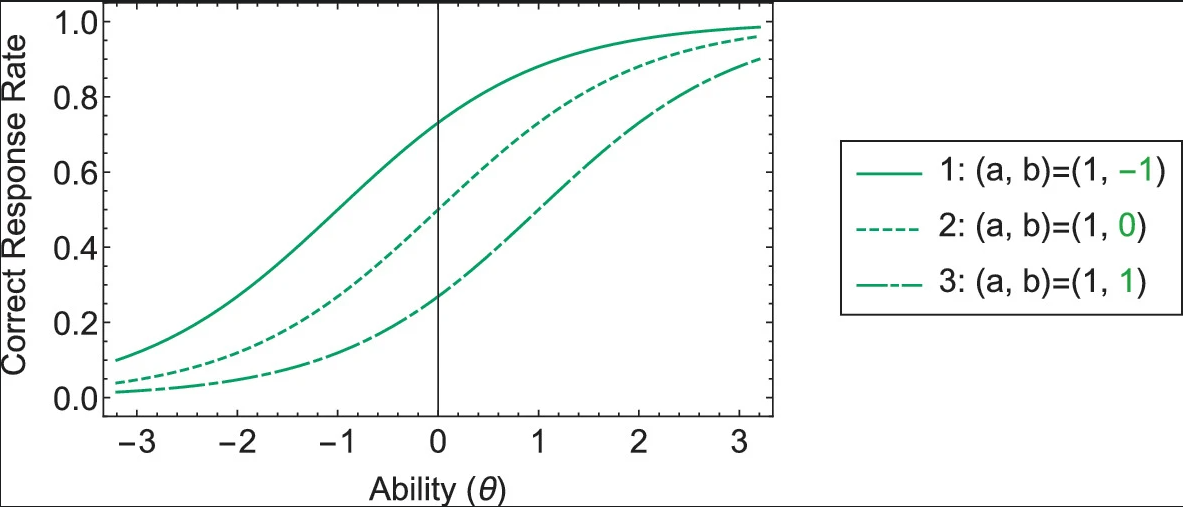
\includegraphics[scale=.5]{imagenes/IRTparambdifficulty.png}
	\caption{Probabilidad de responder correctamente para distintos valores del parámetro dificultad \textit{b}.}
	\label{ParamDifficulty}
\end{figure}


Es importante destacar que cada ítem discrimina mejor en torno a valores de $\theta$ que sean cercanos al parámetro de locación $b$. Además, un parámetro $a$ indica que el item es un mejor indicador para $\theta$, pero teniendo en consideración que este poder discriminativo funciona mejor cuando $\theta \approx b$. Por esta razón, cada pregunta por separado entrega información acerca del valor $\theta$ que se quiere obtener, de manera que las preguntas deben estar formuladas de tal manera que permitan distinguir distintos niveles del rasgo a evaluar \cite{TeoriaRespuestaAlItemPsicologia}.

Aplicando este modelo a una escala de Likert de formato ordinal, para cada pregunta se indican 4 parámetros b, para diferenciar entre los niveles 1) Muy en desacuerdo; 2) En desacuerdo; 3) Ni en desacuerdo ni de acuerdo; 4) De acuerdo y 5) Muy de acuerdo \cite{TeoriaRespuestaAlItemPsicologia, meegaplusQualityEvaluationPage}. De esta manera, a medida que $\theta$, la calidad de juego es mejor según \cite{meegaplusQualityEvaluationPage}, las respuestas más tenderán a ser del formato Muy de acuerdo, a excepción de algunas preguntas que no se incluyen en la valoración. El script de R utilizado para el cálculo de $\theta$ se encuentra disponible en \cite{meegaplusQualityEvaluationPage}.

Las fórmulas empleadas, demostraciones relacionadas con IRT o mostrar cómo afectan los distintos parámetros al resultado final está fuera del alcance de este estudio, principalmente porque los paquetes de R se encargan de realizar este trabajo. Para entender mejor cómo funciona este modelo por debajo, puede consultarse \cite{IRTShojima2022, CalderonStatisticalIRT}.

\subsection{Motores de videojuegos: Godot}

Existen diversos motores de videojuegos, como Unreal Engine \cite{UE}, Unity \cite{Unity} y Godot \cite{Godot}. Este último resalta por ser completamente gratuito, de código abierto y poseer una comunidad activa en el desarrollo del motor \cite{GodotGithubRepository}. Los motores de videojuegos ofrecen una ventaja significativa al proporcionar un entorno integrado que abarca diversas funcionalidades para diferentes profesionales. Por ejemplo, facilitan la integración de animaciones, efectos visuales, y trabajo con sonido. Además, incluyen bibliotecas incorporadas comúnmente utilizadas en videojuegos, como colisiones, texturizado, o composición de elementos, permitiendo la unificación de la representación visual, auditiva y programática de un personaje. Los motores de videojuegos también posibilitan la exportación de la aplicación a diversas plataformas sin necesidad de modificar el código \cite{GodotExport}.

Godot emplea principalmente dos lenguajes de programación: GDScript, similar a Python, y C\#. Ambos fueron utilizados en este trabajo. GDScript permite prototipar rápidamente debido a su simplicidad y estrecha integración con el motor. Por otro lado, C\# es más rápido, pero algunas características del motor no están completamente integradas en la versión utilizada durante este trabajo, que es la 3.5.2 \cite{GodotCSharpGDDifferences}.

\chapter{Trabajo Relacionado}


Un videojuego es una forma de aprendizaje activo, pues el proceso de enseñanza no se desarrolla partiendo por un profesor exponiendo frente a un estudiante. En este caso, quien aprende debe ejectuar pasos y participar en alguna actividad a través de la cual se construye el conocimiento. En la reseña realizada por Hartikainen et al. \cite{active_learning_review} se enumeran justificaciones para el aprendizaje activo:  mejores resultados, recomendaciones políticas y las nuevas demandas de la vida laboral actual, como capacidades de comunicación o descubrimiento por cuenta propia. 

Los videojuegos serios (Serious Gaming) son una forma de aprendizaje activo. Un trabajo de Bell y Gibson \cite{evaluation_of_games_for_teaching_cs} indican que los juegos educacionales son más efectivos que las clases, lecturas, videos y tareas. Se resume que el uso de juegos resulta en 1) mejor retención, 2) mejor conocimiento fáctico, 3) mejor conocimiento basado en habilidades y 4) mayor autoeficacia. Sin embargo, recomiendan que los juegos  deben ser acompañados de otras formas de enseñanza, así como hacer actividades post juego donde se le pregunta al estudiantado cómo se relacionan los juegos a la materia.

Bell y Gibson \cite{evaluation_of_games_for_teaching_cs} identificaron y clasificaron videosjuegos de Ciencias de la Computación (CS), considerando un total de 41 videojuegos. Uno de ellos, Map Coloring, se trata sobre grafos, tomando el tema de coloreo de grafos. Se realizó una búsqueda del juego a la fecha (2022), pero no se encontró ningún material al respecto.

Kiili y su equipo \cite{using_videogames_maths} analizaron el uso de videojuegos en enseñanza y evaluación en matemáticas a través de los títulos ``Semideus'' y "Wuzzit Trouble". A través de estos, llegaron a la conclusión de que es posible utilizar videojuegos para enseñar y evaluar al mismo tiempo. Además, caracterizaron estadísticamente las diferencias producidas por el uso de videojuegos entre resultados de un pre test y un post test.

En el trabajo realizado por Zhao y Shute \cite{video_game_foster_computational_thinking} se enumeran ejemplos de videojuegos pensados para enseñar programación, tales como Wu's Castle \cite{wuscastle}, CodeCombat \cite{CodeCombat}, CodeSpell \cite{codespells}, MiniColon \cite{minicolon}, tales ejemplos utilizan programación con texto. Sin embargo, también hay numerosos ejemplos que utilizan programación por bloques, como LightBot \cite{LightBot}, Scratch \cite{maloney2010scratch}, \cite{scratch} y RoboBuilder \cite{RoboBuilder}, los cuales abstraen el trabajo de aprender una sintaxis relacionada a los lenguajes de programación.

Sin embargo, el impacto de estos videojuegos no ha sido evaluado en muchos casos. En los casos documentados, se cuenta con muestras pequeñas, además de que se trata principalmente de evaluaciones puramente cualitativas \cite{video_game_foster_computational_thinking}, \cite{effectiveness_gbl}.

Kiili y su equipo, Bell et al., Giani y otros \cite{petri2018method} están de acuerdo en que no hay sistematización en la evaluación de videojuegos educativos. En efecto, hay juegos serios que ni siquiera se denominan o consideran como tales \cite{evaluation_of_games_for_teaching_cs}. Por otra parte, no existe una forma estándar de evaluarlos, razón por la cual Petri, Giani y otros \cite{petri2018method} crearon el modelo MEEGA+ (Model for the Evaluation of Educational Games and EGameFlow scale).

Entre las faltas mencionadas al momento de crear videojuegos, se mencionan las faltas de 1) Definición de un objetivo de evaluación; 2) Diseño de investigación; 3) Programa de medición; 4) Instrumentos de recolección de datos y 5) Métodos de análisis de datos. Un ejemplo de falta de sistematización: una práctica común al analizar estas herramientas son los comentarios informales por parte del estudiantado \cite{petri2018method}.






\chapter{Diseño de la Solución}

% Contenidos basados en https://repositorio.uchile.cl/bitstream/handle/2250/191381/TablaConten.pdf?sequence=2&isAllowed=y
La aplicación creada, llamada IGACSE (Interactive Graph Algorithms for Computer Science Education) de ahora en adelante, es propuesta y diseñada en base a algunos requerimientos y necesidades de los estudiantes de computación que se nombrarán en las siguientes secciones.

\section{Referentes}

Los referentes más importantes son aquellos videojuegos que tienen un rol educativo relacionado a la programación, como CodeCombat \ref{CodeCombat} y 7 Billion Humans \ref{7BillionHumans}.

Se observa que estos juegos tienen una componente textual que destaca en la interfaz del juego principal, ocupando al menos el 20\% de la pantalla. Por otra parte, hay texto que avanza en una línea narrativa al inicio y final de cada nivel.

En ambos casos la interfaz de código se encuentra a la derecha. Además, estos juegos permiten mostrar al usuario cómo la ejecución de las instrucciones afecta al juego paso a paso.

De este análisis se desprende que el juego tiene por requisito mostrar la ejecución del código instrucción por instrucción.

\section{Objetivo del diseño deseado}

En este apartado se justifican las decisiones de diseño que llevaron a las mecánicas de juego, cuáles son los elementos interactivos y la ubicación y responsividad de estos. Según Rogers en su libro sobre diseño interactivo \cite{Rogers2002InteractionDesign}, es relevante entender primero cuál es el problema que busca resolverse, qué usuarios se ven afectados por esto, qué características poseen y cómo podría solucionarse en base a prototipos.

Se parte del supuesto de que, en muchas ocasiones, los estudiantes creen entender cómo funciona cierto código o algoritmo, pero no lo aplican paso a paso con papel y lápiz o en su imaginación propia. Cuando se les asigna como ejercicio realizar el procedimiento siguiendo cada instrucción rigurosamente, los estudiantes no lo llevan a cabo o lo hacen de forma incorrecta sin darse cuenta. Por ejemplo, en \cite{IdentifyingStudentDifficultiesDataStructures}, se menciona que los estudiantes a menudo creen entender los contenidos, pero tienen conceptos erróneos sin percatarse.

En el trabajo de Zingaro et al. \cite{IdentifyingStudentDifficultiesDataStructures}, se mencionan algunos ejemplos de malentendidos por parte de los estudiantes, como errores al comprender los heaps y las formas en que pueden representarse o construirse. Estos malentendidos pasan desapercibidos y no son detectables por los mismos estudiantes.

Adicionalmente a la revisión de textos, se revisaron canales de YouTube educativos como 3Blue1Brown \cite{3Blue1BrownYT}, donde el propietario del canal, Grant Sanderson, habla repetidamente sobre cómo las visualizaciones ayudan a comprender la abstracción matemática subyacente.

Un requisito esencial es que el videojuego logrado debe evitar la mecanización por parte del estudiante, obligándolo a revisar exhaustivamente cada paso relacionado con el algoritmo, evitando dar por sentado que se entiende el código y saltar a la siguiente actividad.

Por otra parte, para enseñar conceptos relacionados con programación, lo ideal es buscar usuarios que entiendan cómo funciona, pero que no tengan mucha experiencia y que no visualicen un código al nivel de entender cómo funciona instrucción por instrucción. Por lo mismo, se propone basarse en un modelo similar a los debuggers, donde se puede ver el estado de las variables en cada paso, así como la instrucción por ejecutarse y el resultado que conlleva.

\section{Descripción de la aplicación al momento de la realización de los experimentos}

El videojuego se separa en distintos niveles. Consta de un menú principal, tutoriales y niveles jugables. En el menú principal se puede seleccionar el nivel a jugar o un modo historia. En el modo historia, se juegan todos los niveles en orden, y se desbloquean a medida que se avanza.

En los tutoriales se abordan los conceptos básicos de grafos sin indicar explícitamente al usuario qué es un grafo. Además, se enseñan conceptos de jugabilidad, como explorar o seleccionar un nodo, navegar en el código ejecutando instrucciones y responder preguntas del tipo Sí/No cuando el código incluye una instrucción con un if.

Finalmente, se presentan los niveles jugables, correspondientes a los algoritmos que se buscan enseñar: BFS (Breadth First Search) y DFS (Depth First Search). En estos niveles, no se presenta una historia y hay menos ayuda para el usuario. Una vez completados los niveles jugables, se mostrarán los créditos del juego.

El juego se centra en explorar planetas a través de rutas, utilizando una metáfora de grafos, donde los planetas representan nodos y los caminos entre ellos son aristas. El objetivo es rescatar pandas rojos dispersos en los planetas. Para lograrlo, es necesario explorar todos los nodos en una galaxia, correspondiente a un nivel. En cada nivel, se enseña un algoritmo distinto.

El juego guía al usuario mediante instrucciones que aparecen en el lado derecho de la pantalla. El jugador pasa a la siguiente instrucción presionando la tecla de espacio. Cada vez que avanza a la siguiente instrucción, se desencadenan efectos y animaciones que muestran qué está sucediendo en el código. Estas animaciones se reflejan en el viewport del juego, donde se destaca un planeta, un camino o una nave que se desplaza hacia otro planeta.

En los tutoriales se enseñan los conceptos básicos de grafos, pero sin indicarle al usuario explícitamente qué es un grafo. Además, se enseñan conceptos de jugabilidad, cómo explorar o seleccionar un nodo, cómo navegar en el código ejecutando instrucciones, y cómo contestar preguntas del tipo Sí/No cuando el código tiene una instrucción que incluya un if.

Al seguir las instrucciones en su totalidad, el jugador repite el algoritmo paso a paso, lo que le permite entender cómo funciona y cuál es su finalidad.

Las acciones del jugador pueden ir acompañadas de un sonido recompensante, permitiéndole avanzar a la siguiente instrucción. En caso de cometer un error, se indicará al jugador mediante una animación visual y un sonido. Si el jugador no sabe qué hacer, en ciertos casos se mostrará un hint visual indicándole que debe presionar alguna tecla específica o hacer clic en algún planeta.


\subsection{Diagrama de flujo de juego}

El juego inicia mostrando el menú principal, donde se puede seleccionar el modo historia o los niveles jugables. Si se elige el modo historia, se mostrarán los tutoriales. Una vez terminados los tutoriales, se mostrará el primer nivel jugable, que es DFS. Si se eligen los niveles jugables, se mostrarán los niveles jugables, donde se puede seleccionar el nivel a jugar, BFS o DFS.
Terminados los niveles BFS y DFS, se mostrarán los créditos.

\begin{figure}[h]
	\centering
	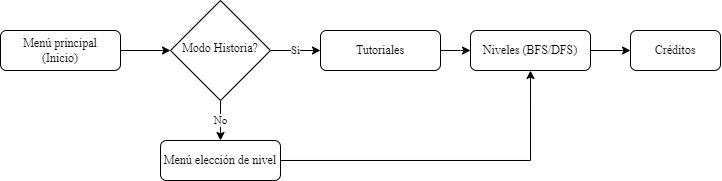
\includegraphics[scale=.5]{imagenes/FlujoDeJuego.png}
	\caption{ Flujo de juego de IGACSE}
	\label{FlujoDeJuego}
\end{figure}


\subsection{Narrativa}

La narrativa se desarrolla en el espacio exterior, donde una nave inicia un diálogo con una estación llamada DCC. La misión de la nave es rescatar pandas rojos dispersos en los planetas de la galaxia. En un inicio, el piloto señala que los niveles de combustible son bajos, y la estación sugiere continuar con las siguientes galaxias, evitando el uso del piloto automático debido al alto costo y consumo de combustible de las redes neuronales. Para optimizar recursos, la nave deberá seguir instrucciones manuales para completar la misión.

Con cada galaxia visitada, el piloto rescata y encuentra otros pandas rojos. Se premia al jugador para que siga con los siguientes niveles y que termine el juego. Los pandas rojos son la mascota del Centro de Alumnos del Departamento de Ciencias  de la Computación (CADCC).  Durante las actividades de bienvenida a los nuevos estudiantes, se muestran afiches con esta mascota \cite{CADCCPage}, por lo que se busca que el jugador se sienta identificado con el juego. Además, la estación se llama DCC para aumentar el sentido de identificación con el jugador, pues DCC son las siglas del Departamento de Ciencias de la Computación \cite{DCCPage}.


\subsection{Menú principal}

En el menú principal, se puede seleccionar el idioma presionando el botón en la esquina superior izquierda de la figura \ref{MenuPrincipal}. Los idiomas disponibles son inglés y español. Además, ofrece las opciones para jugar en el modo historia o los niveles jugables.

\begin{figure}[h]
	\centering
	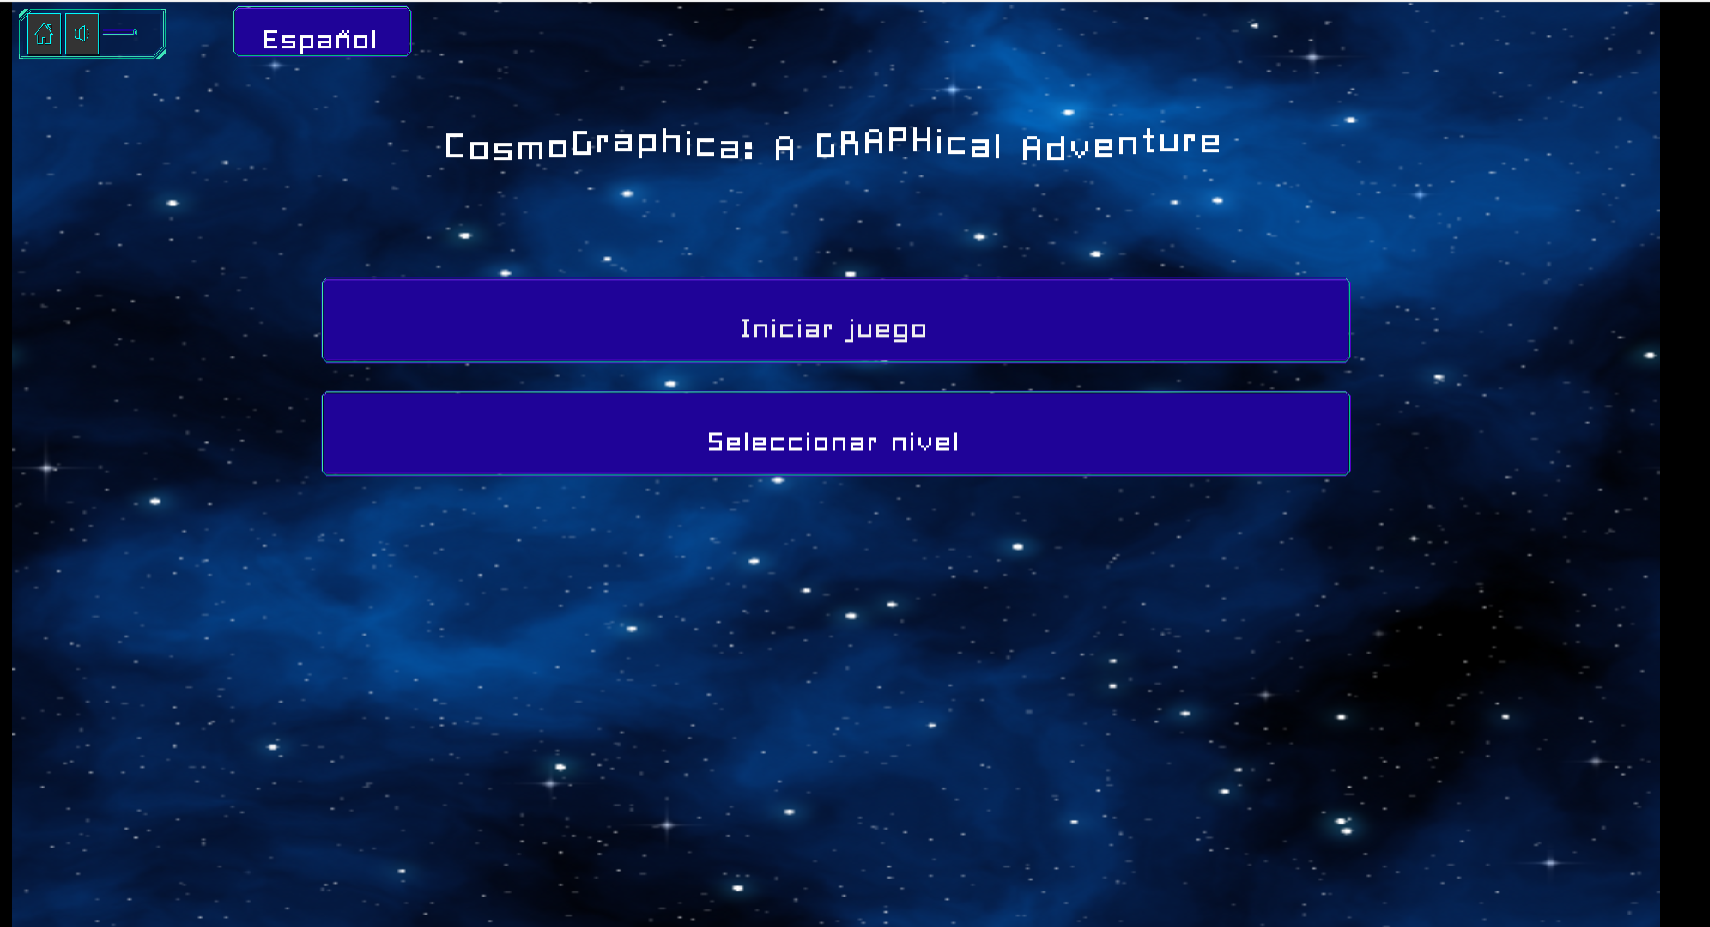
\includegraphics[scale=0.3]{imagenes/MainMenu.png}
	\caption{Menú principal de IGACSE, que se muestra al iniciar el juego.}
	\label{MenuPrincipal}
\end{figure}


\subsection{Tutoriales}

Los tutoriales tienen como objetivo familiarizar al jugador con las mecánicas básicas que se utilizarán a lo largo del juego. Además, introducen al jugador en la historia, ambientada en una nave que rescata pandas rojos dispersos en los planetas de la galaxia. La trama busca ilustrar la aplicación de los grafos sin detallar explícitamente el contenido que se está enseñando. Las mecánicas se presentan mediante una combinación de elementos, como texto y pistas visuales, que pueden incluir un ratón realizando clic izquierdo o una tecla R siendo presionada sobre el planeta. Cada nivel y tutorial son repetibles, permitiendo al jugador revisarlos en caso de no comprender algún aspecto.

\subsubsection{Primer Tutorial}

En el primer tutorial, se pretende familiarizar al jugador con la pantalla, demostrando que los planetas son navegables y que existen caminos que los conectan, permitiendo hacer clic entre ellos. En esta etapa, también se proporciona información sobre el diálogo y se presentan pistas visuales.


\begin{figure}[h]
	\centering
	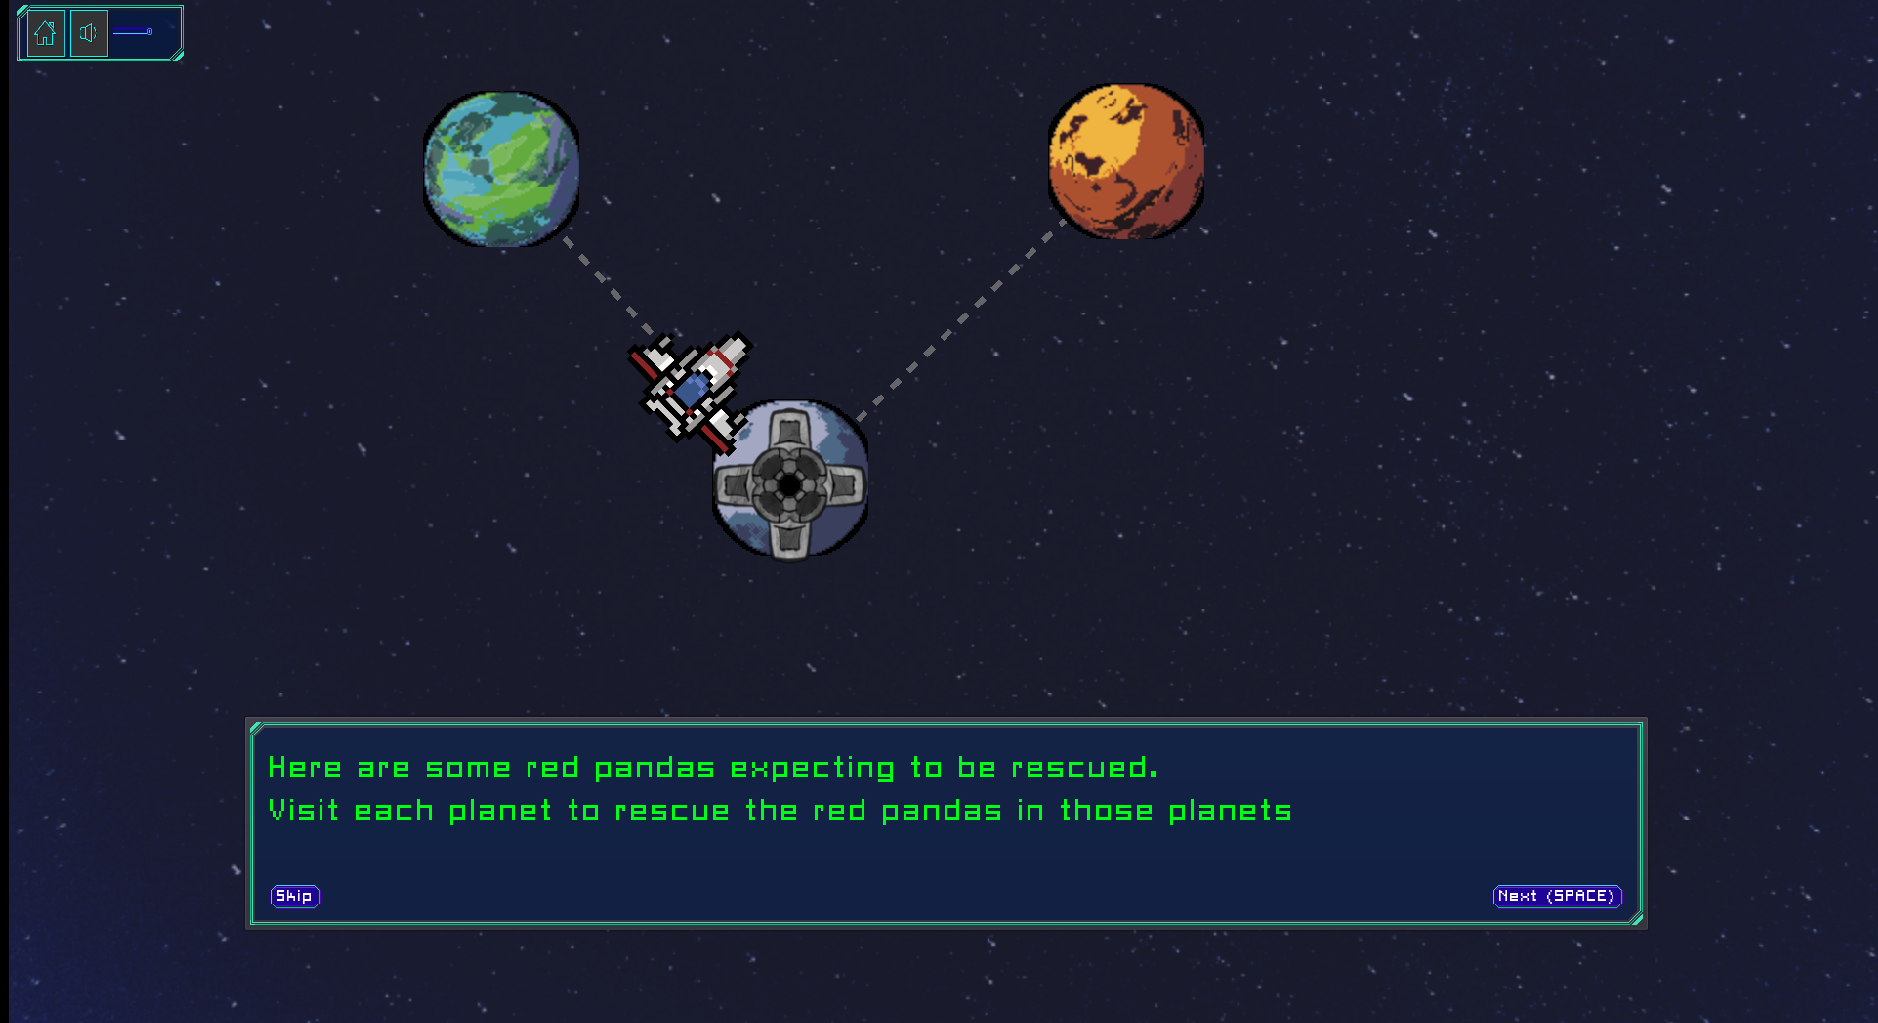
\includegraphics[scale=0.3]{imagenes/FirstTutorial.png}
	\caption{Primer tutorial. Se le indica al jugador a través de un diálogo que debe visitar cada planeta.}
	\label{FirstTutorial}
\end{figure}



\subsubsection{Segundo tutorial}

En el segundo tutorial, se presenta la mecánica de instrucciones e introduce el ciclo for y el if en las instrucciones, elementos que se utilizarán más adelante.

Al inicio del segundo tutorial, se le indica al jugador que debe seguir las instrucciones del algoritmo debido a que la exploración automatizada de los pandas rojos es costosa y el combustible se está agotando. Las primeras dos instrucciones solicitan al jugador que presione la tecla espacio para avanzar a la siguiente instrucción (ver figura \ref{SecondTutorial}).


\begin{figure}[h]
	\centering
	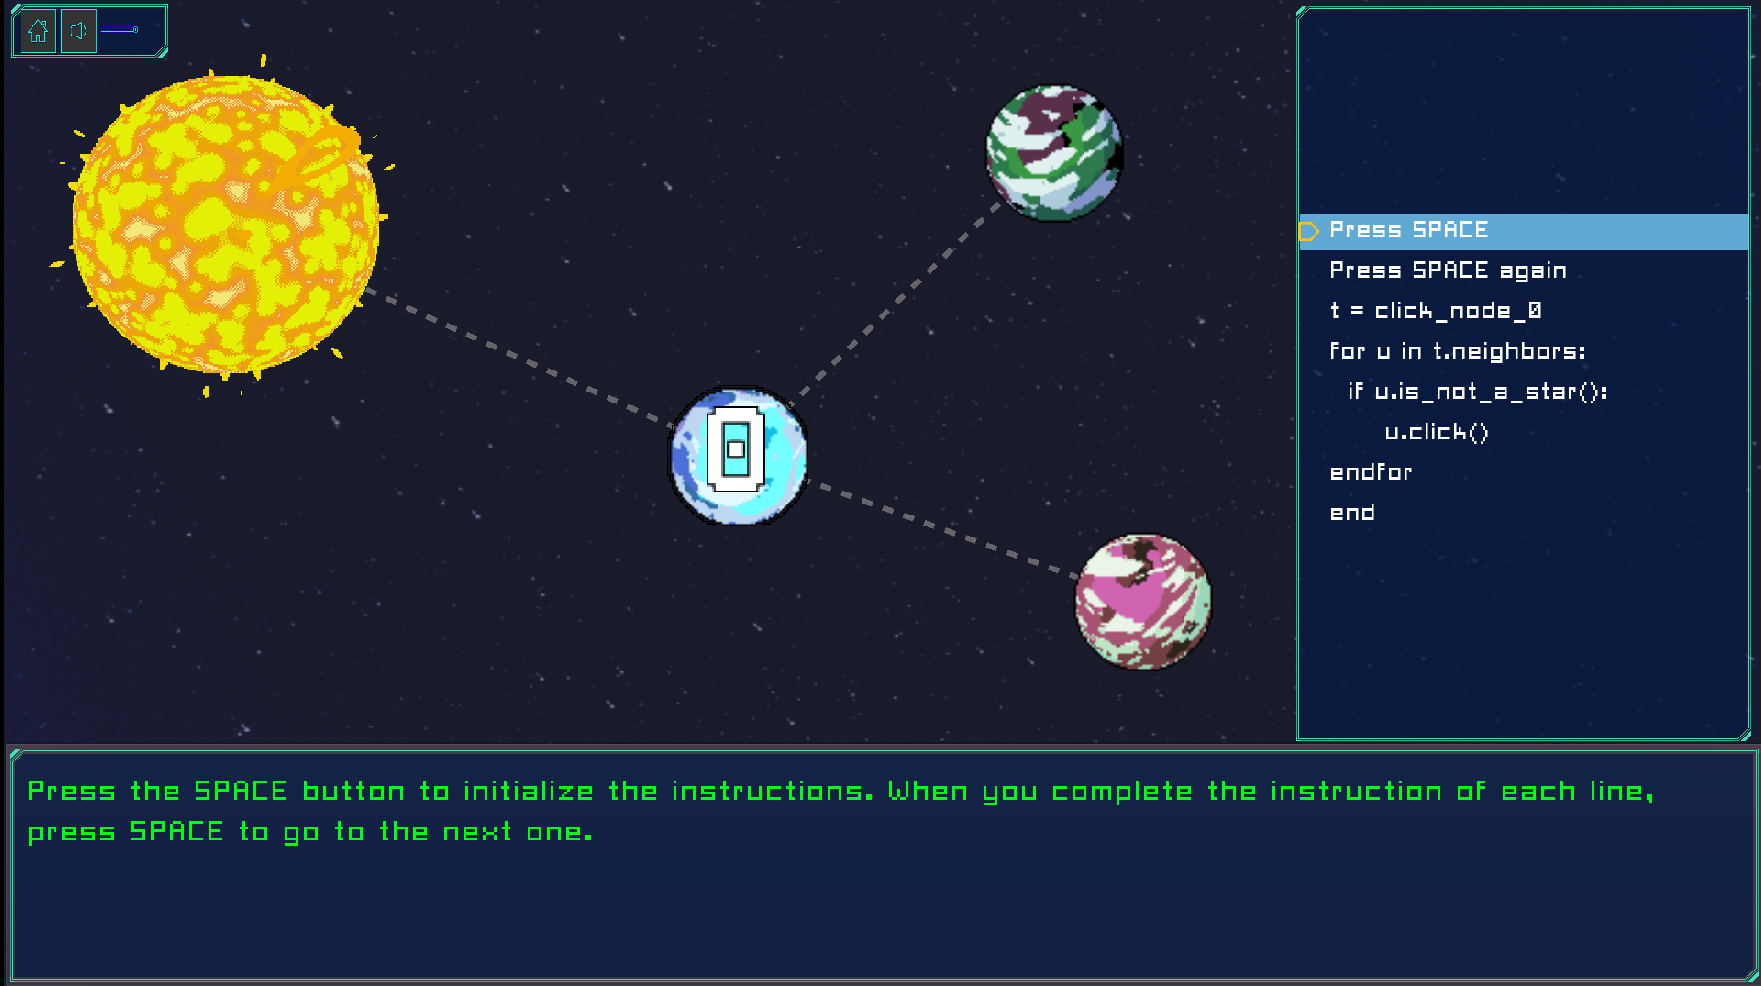
\includegraphics[scale=0.2]{imagenes/SecondTutorial.png}
	\caption{Segundo tutorial. Se le muestra un diálogo de entrada al jugador introduciéndole el nuevo concepto. Este es el primer momento en que se le muestran las instrucciones al jugador.}
	\label{SecondTutorial}
\end{figure}

Durante este segundo tutorial, se introduce la lógica de responder sí o no cuando aparece una instrucción con un if. El jugador debe dar la respuesta correcta para avanzar a la siguiente instrucción. Si responde incorrectamente, perderá y deberá reiniciar el nivel. En la figura \ref{SecondTutorialShowingIf}, se muestra la ventana que aparece al jugador al llegar a una instrucción con un if.

\begin{figure}[h]
	\centering
	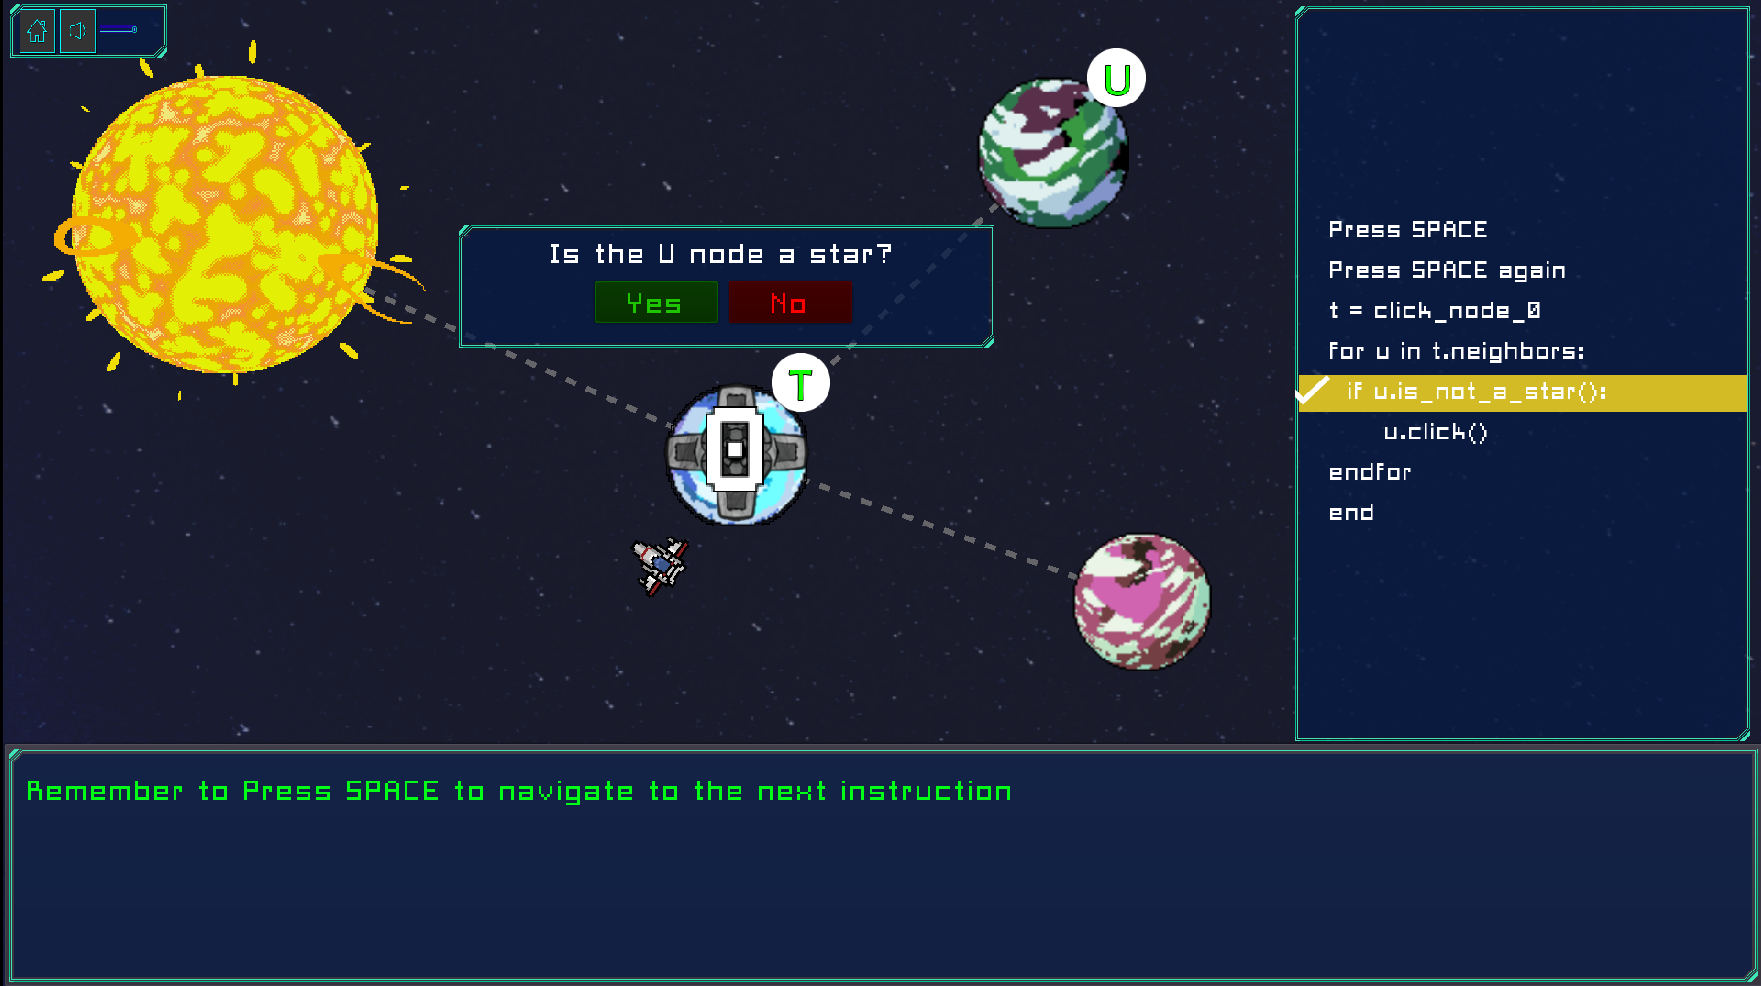
\includegraphics[scale=0.3]{imagenes/SecondTutorialShowingIf.png}
	\caption{Segundo tutorial. Ventana de if que le aparece al jugador al llegar a una instruccion con un if. El jugador debe responder sí o no correctamente para avanzar}
	\label{SecondTutorialShowingIf}
\end{figure}

\subsubsection{Tercer tutorial}

El tercer tutorial introduce al jugador el concepto de Pilas (Stacks) y Colas (Queues) como estructuras de datos para almacenar nodos y luego obtenerlos en órdenes distintos. Además, se le introduce al jugador sobre las variables creadas y la variable seleccionada, la cual se usa para señalar a qué objeto se le agregará el nodo que el usuario presione.

\begin{figure}[h]
	\centering
	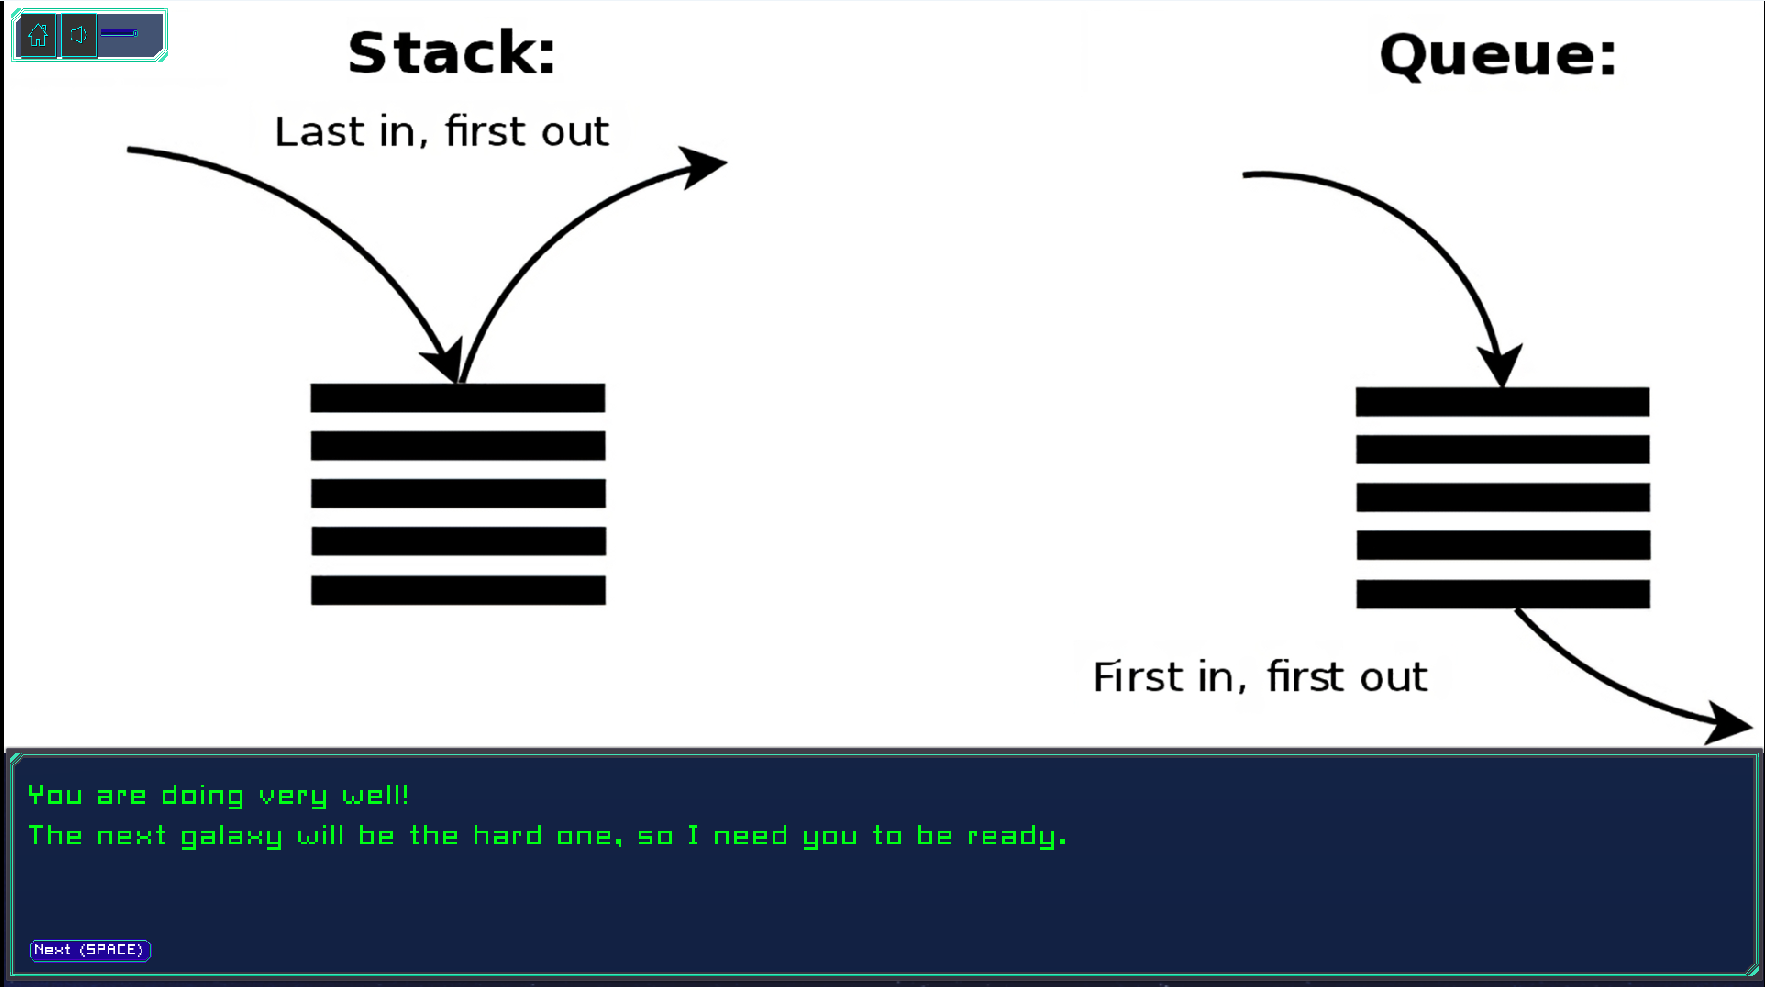
\includegraphics[scale=0.3]{imagenes/ThirdTutorialFirstDialogue.png}
	\caption{Tercer tutorial. Se le explica al usuario al inicio qué son las colas y stacks y cómo funcionan y en qué difieren.}
	\label{ThirdTutorialFirstDialogue}
\end{figure}


\begin{figure}[h]
	\centering
	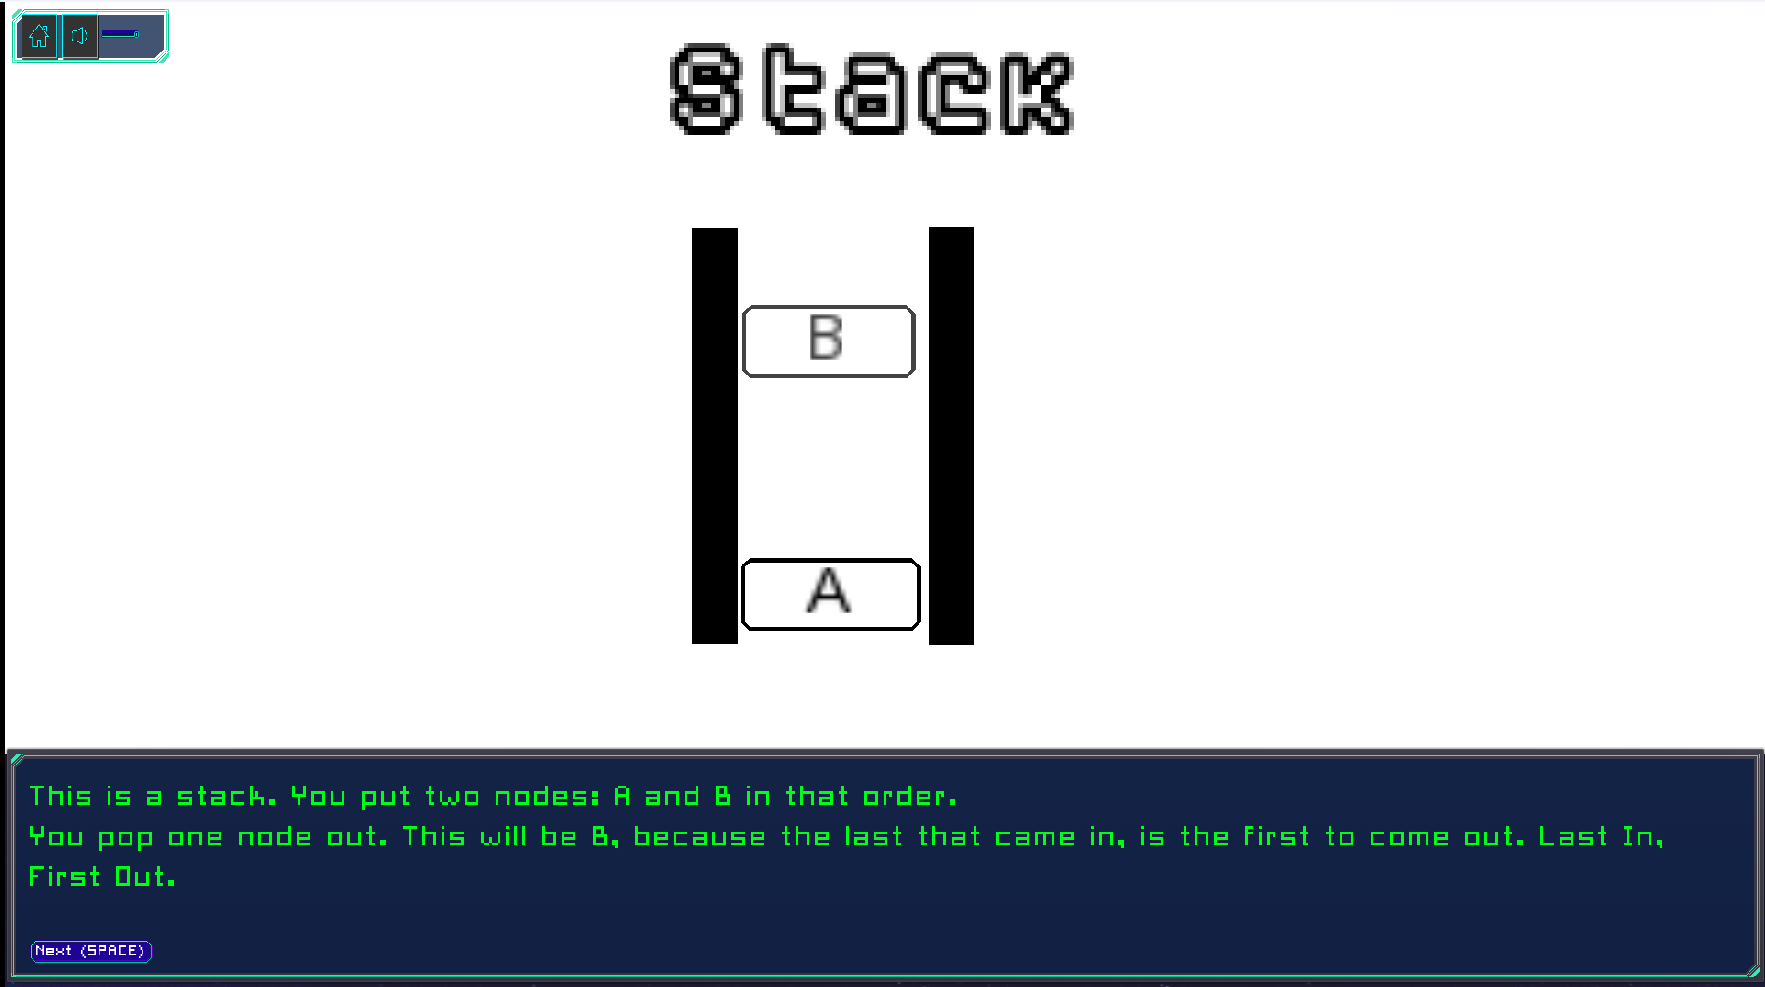
\includegraphics[scale=0.3]{imagenes/ThirdTutorialStackExplanation.png}
	\caption{Tercer tutorial. Mostrando al usuario cómo funciona un stack a través de animaciones.}
	\label{ThirdTutorialStackExplanation}
\end{figure}


El objetivo de las instrucciones en este tutorial es que el jugador aprenda la mecánica para agregar nodos a un stack o a una pila. Además, se refuerza la mecánica de las instrucciones y ejecutar cada acción paso por paso.


\begin{figure}[h]
	\centering
	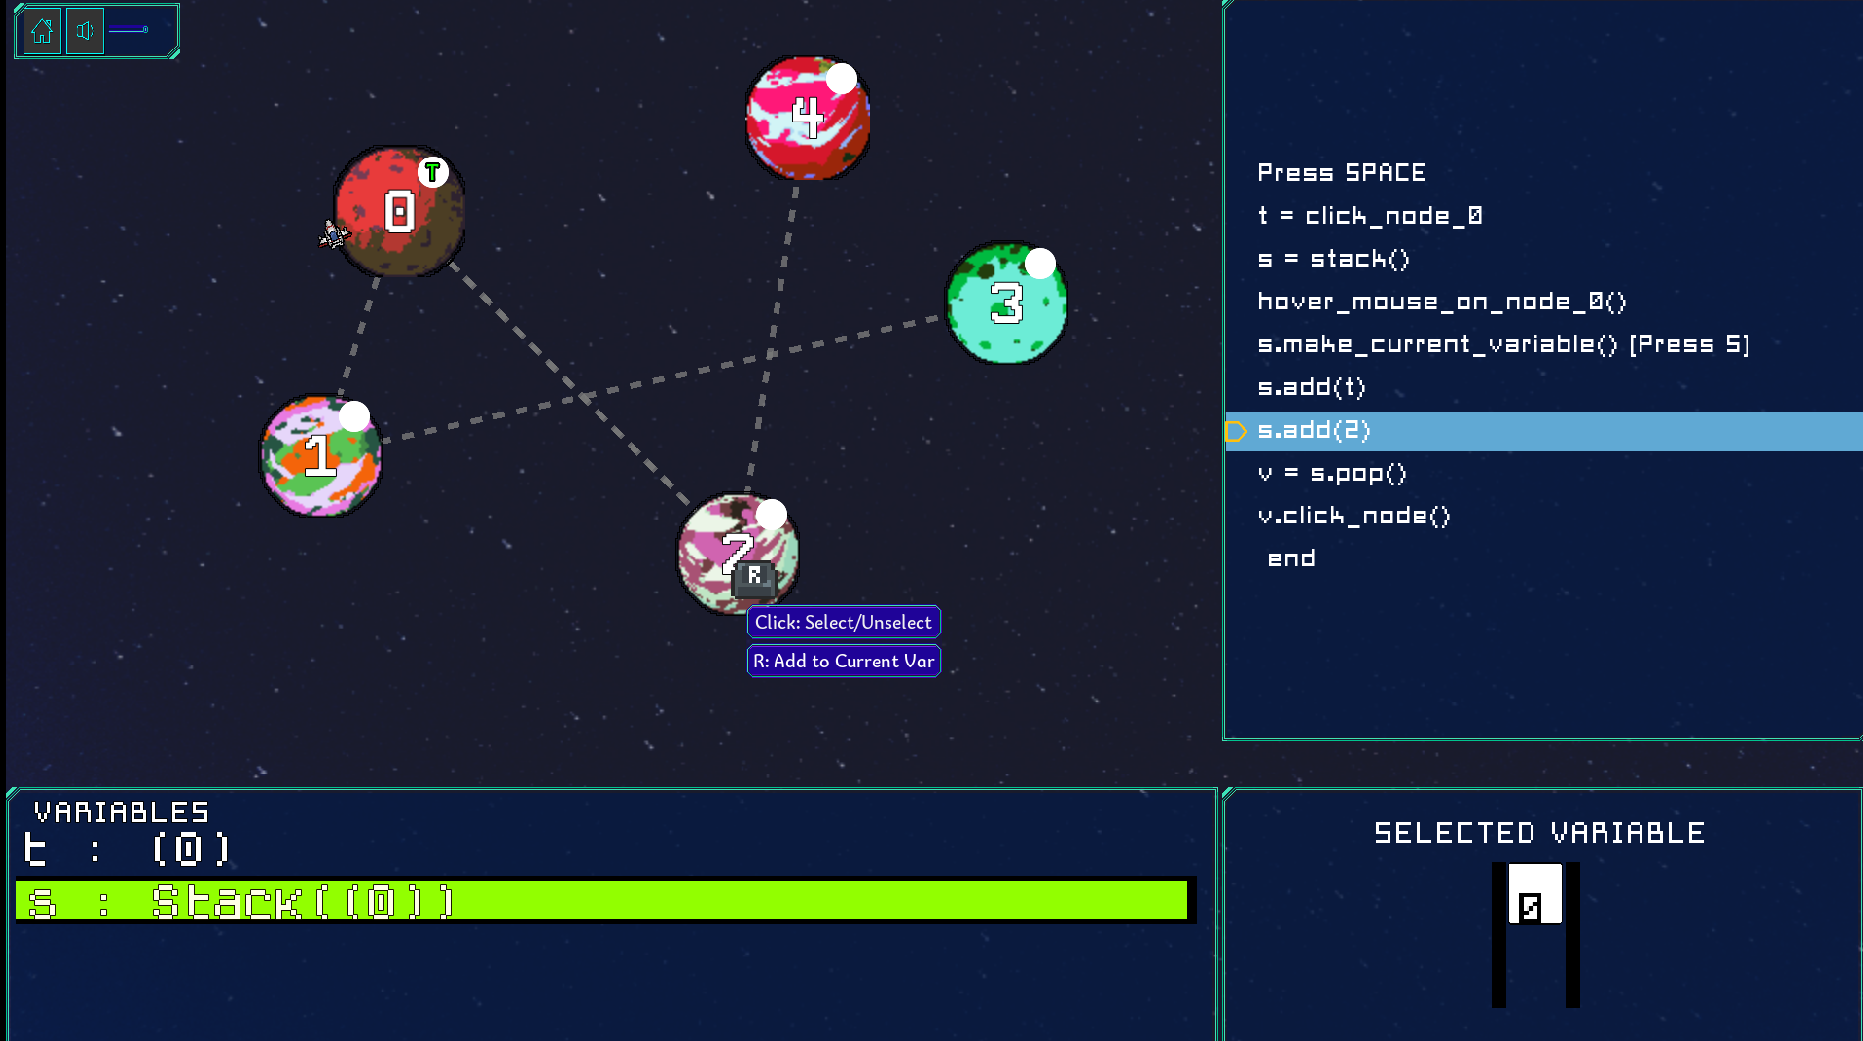
\includegraphics[scale=0.3]{imagenes/ThirdTutorialAddingNode.png}
	\caption{Tercer tutorial. El jugador debe presionar R sobre el planeta 2 para avanzar a la siguiente instrucción.}
	\label{ThirdTutorialAddingNodesToStacks}
\end{figure}


\subsection{Niveles jugables}

Los niveles jugables presentados son BFS y DFS, que enseñan esos algoritmos. Los planetas y sus conexiones son aleatorias, con la restricción de que el grafo formado es siempre conexo, es decir, todos sus nodos tienen al menos un camino hacia el resto de los otros nodos.

Se crearon 4 niveles para el juego, incluyendo los algoritmos de Kruskal y Prim. Sin embargo, estos últimos no fueron incluidos en la versión final del juego, pues el diseño y la experiencia de usuario eran distintos por requerir otro tipo de acciones, como ordenar arcos y operar con conjuntos, obteniendo uniones e intersecciones. Además, el tiempo de la prueba de usuario era aproximadamente de 45 minutos, por lo que se prefirió no incluirlo en la prueba dado que no se contaba con el tiempo suficiente para probarlos.


\section{Proceso de diseño}

Para diseñar el videojuego, primero se determinaron problemas que se querían solucionar. En particular, el autor hipotetiza que los estudiantes de computación tienen dificultades para comprender completamente los algoritmos que se enseñan en los cursos de programación, y que no siempre son conscientes de esta falta de comprensión. Por lo tanto, se busca que este videojuego sea una herramienta que permita a los estudiantes entender los algoritmos paso a paso, guiándolos sutilmente a lo largo del proceso de aprendizaje.

En la Universidad de Chile, históricamente y al momento de realizar este trabajo, para entrar a computación se requiere aprobar anteriormente dos años de cursos de plan común, donde existe una práctica conocida como ``pauteo'', la cual consiste en estudiar y revisar pautas de pruebas de semestres pasados para preparase para los exámenes. Con esta práctica, el alumnado revisa las ecuaciones o procedimientos para responder una pregunta sin haber realizado los ejercicios o repetido el procedimiento paso por paso. Muchas veces revisan un algoritmo superficialmente, o lo reproducen mentalmente sin hacerlo en papel. Por lo mismo, se busca que el videojuego sea una herramienta que permita a los estudiantes entender los algoritmos paso a paso y acompañarlo con una visualización.

La idea principal es forzar al usuario a reproducir el algoritmo paso a paso. Esto se puede observar al utilizar el debugger. El debugger permite ver el estado de las variables en cada paso, y permite avanzar paso a paso en el código. El videojuego busca ser una herramienta que permita al usuario reproducir el algoritmo paso a paso, pero de una manera más lúdica. Por esto, el debugger que se utiliza en Visual Studio Code se utilizó como modelo.

% Agregar imagen de debugger en VSCode con un código de Python.

Posteriormente, se realizaron distintos bocetos. Se le mostraron estos bocetos a un diseñador de videojuegos profesional con títulos ya liberados. Se eligió el que fue entendido a primera vista y que se veía más atractivo, además que se parecía más a Visual Studio Code. Se implementaron versiones del videojuego con Godot, que permitía agregar nuevas funcionalidades rápidamente, además de permitir cambiar el estilo. El autor del trabajo mostraba su trabajo de tesis semana a semana en un curso de 20 estudiantes, donde se recibían comentarios del resto de los alumnos.

Una vez definido cierto nivel de avance con todos los algoritmos definidos, se probó con 4 usuarios expertos que ya conocían el algoritmo. Sin embargo, no fueron capaces de seguirlo o comprenderlo a cabalidad, por lo que no se cumpliría el objetivo con personas neófitas en los grafos. Por esta razón, se decidió conseguir la asesoría directa de un diseñador de videojuegos y un diseñador de UX/UI.

Los diseñadores, en entrevistas separadas coincidieron en la necesidad de introducir tutoriales que mostraran los elementos del juego uno a uno, por lo que se decidió agregar tutoriales. Además, se decidió agregar una historia de fondo para lograr que el jugador se sienta identificado con el juego y comprenda un uso inmediato de estos algoritmos y estructuras. Por otra parte, los diseñadores enfatizaron la necesidad de agregar una componente de premiación y gamificación para despertar la motivación de los usuarios.

Una vez finalizados los tutoriales, junto con la incorporación de los estilos, música y elementos narrativos, se procedió a publicar \href{https://alasaltum.itch.io/igasce}{el videojuego en la plataforma de itch.io}, un servidor de venta de videojuegos y elementos relacionados de creadores con bajos recursos o del mundo indie. El estilo se compró en itch.io a través de la \href{https://azagaya.itch.io/sci-fi-theme}{tienda de assets}. Los sonidos también se descargaron desde la misma tienda.

% Agregar fotos de distintas versiones del juego
% TODO: podríamos mostrar el proceso de diseño, con las distintas evoluciones.

\subsection{Diseño de la interfaz de usuario}

La interfaz de usuario está basada principalmente en el debugger de Visual Studio Code \cite{vscode} (Ver figura \ref{VScodeDebugger}). Se observa aquí que la instrucción actual está destacada por un puntero y en color. Además, las variables locales muestran su valor en un formato "nombre: valor". El usuario puede avanzar paso a paso en el código.

\begin{figure}[h]
	\centering
	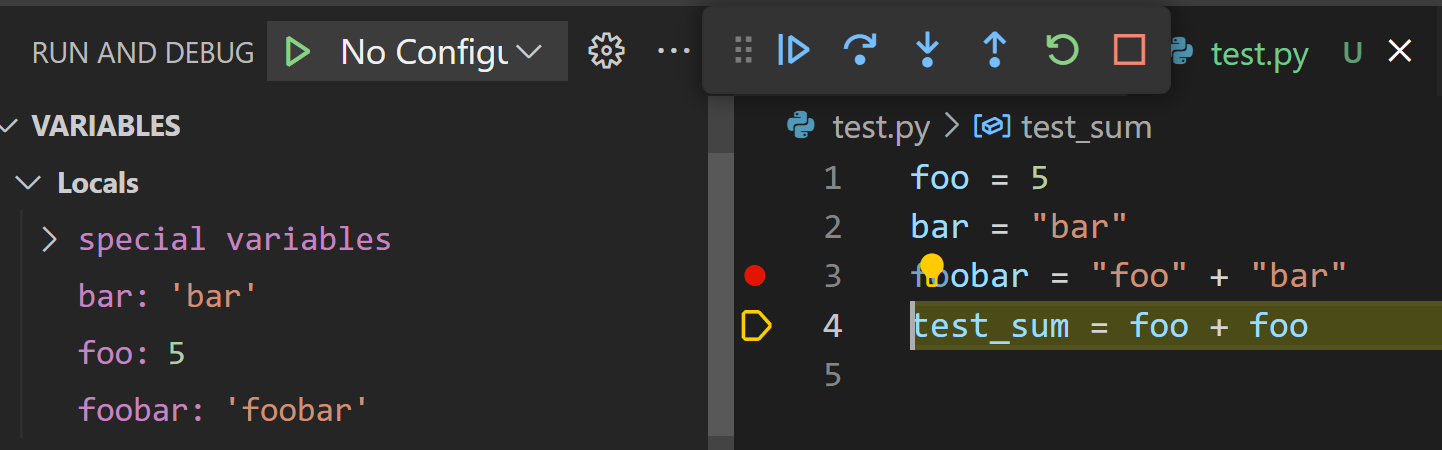
\includegraphics[scale=0.3]{imagenes/VScodeDebugger.png}
	\caption{Visual Studio Code Debugger.}
	\label{VScodeDebugger}
\end{figure}

Hay otros juegos cuya interfaz sirvió de inspiración para la realización del juego final, como 7 Billion Humans\cite{7billionhumans}, donde el código se ve a la derecha de la pantalla. La porción que contiene los elementos y eventos del juego está al lado izquierdo. Lo que ocurre en la interfaz de la derecha afecta al mundo virtual, tal como en la aplicación IGASCE.

\begin{figure}[h]
	\centering
	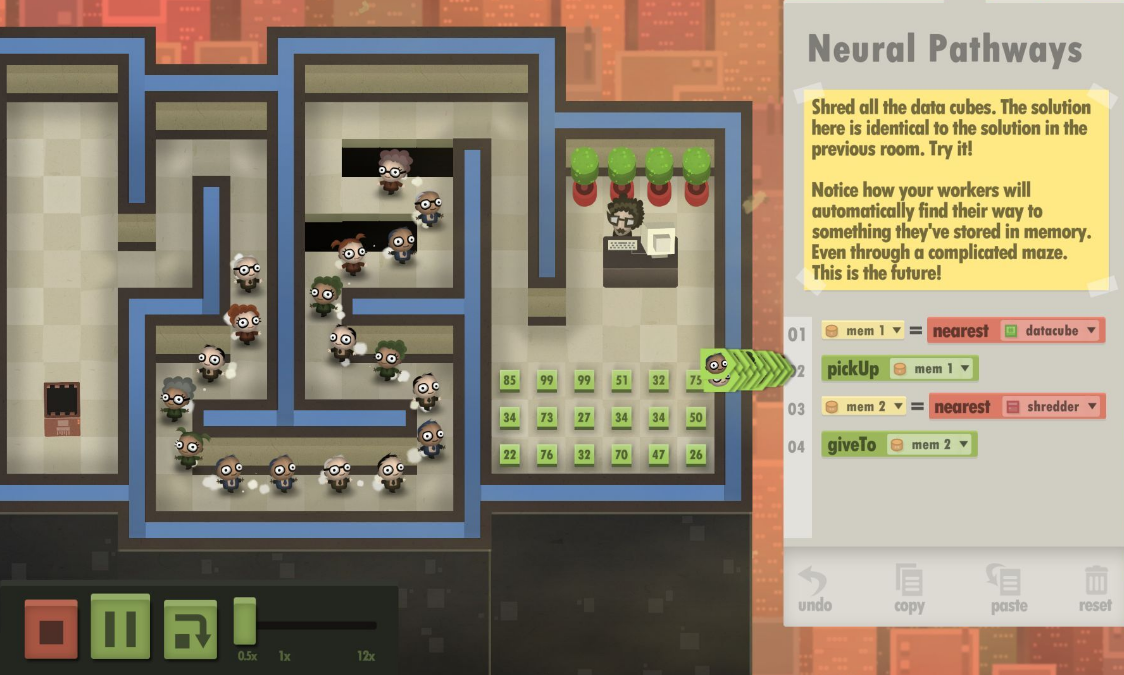
\includegraphics[scale=0.3]{imagenes/7BillionHumans.png}
	\caption{Videojuego 7 Billion Humans}
	\label{7BillionHumans}
\end{figure}


Otro videojuego con una interfaz similar es CodeCombat \cite{CodeCombat}. Aquí el código también está a la derecha, mientras que abajo se ven diálogos y elementos seleccionables. En el caso de IGASCE, los diálogos también se muestran abajo, así como las variables actuales y la seleccionada.
Además, el menú del juego se accede en la esquina superior izquierda (Ver figura \ref{CodeCombat}).

\begin{figure}[h]
	\centering
	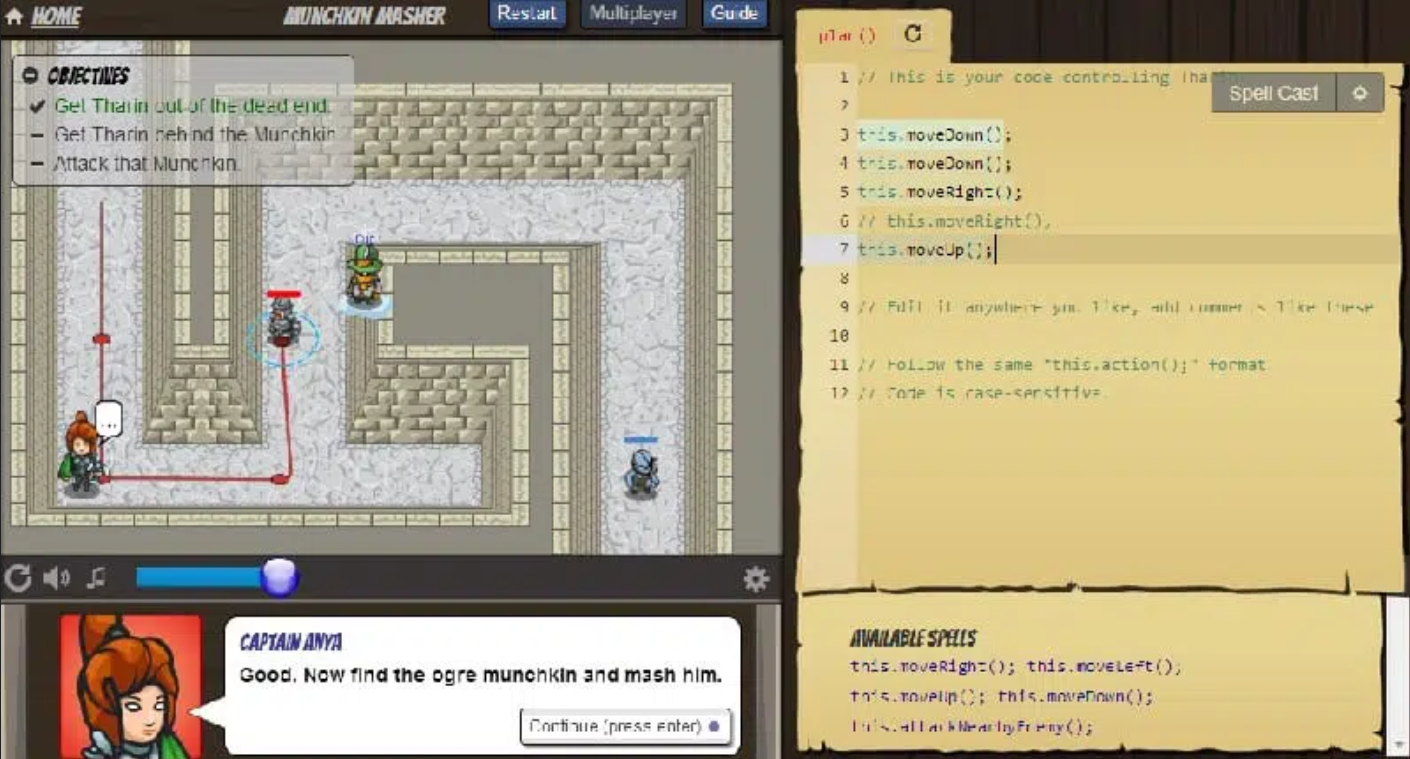
\includegraphics[scale=0.3]{imagenes/CodeCombat.png}
	\caption{Videojuego CodeCombat}
	\label{CodeCombat}
\end{figure}


\subsection{Diseño de efectos de sonido y música}

Los juegos retro comúnmente emplean bucles de música de 8 a 16 bits. Ejemplos notables incluyen Golden Sun \cite{Wiki_Golden_Sun}, ProtoCorgi \cite{ProtoCorgi}, Pokemon Emerald \cite{PokemonEmerald}, Space Invaders \cite{SpaceInvaders}, y Final Fantasy IV \cite{FinalFantasyIV}.

En juegos como Pokemon \cite{PokemonEmerald} y Golden Sun \cite{Wiki_Golden_Sun}, cada vez que se hace click en algún botón y se gatilla un evento, se emite un sonido de confirmación, como cuando el jugador selecciona un ataque. El objetivo es confirmarle al usuario que se está ejecutando correctamente una acción. IGASCE sigue una estrategia similar, utilizando sonidos agudos de confirmación al hacer clic en planetas, caminos o al presionar teclas correctamente (espacio o R). Estos sonidos nítidos cumplen la función de validar la ejecución exitosa de una acción sin distraer al jugador.

En contraste, los sonidos de error en IGASCE emplean tonos graves con desvanecimiento, generando una sensación de vibración (ver figura \ref{EspectroOndasSonidoError}). Estos sonidos más intensos se activan cuando el jugador comete errores, como hacer clic en un planeta incorrecto o un camino equivocado, presionar una tecla antes de completar una instrucción, o responder incorrectamente a preguntas del tipo Sí/No. La intención es que el jugador reconozca inmediatamente los errores y tome medidas correctivas.

\begin{figure}[h]
	\centering
	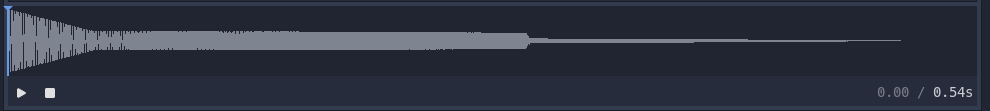
\includegraphics[width=0.9\textwidth]{imagenes/EspectroOndasConfirmacion.png}
	\caption{Espectro de Ondas del sonido de Confirmación de IGASCE}
	\label{EspectroOndasSonidoConfirmacion}
\end{figure}


\begin{figure}[h]
	\centering
	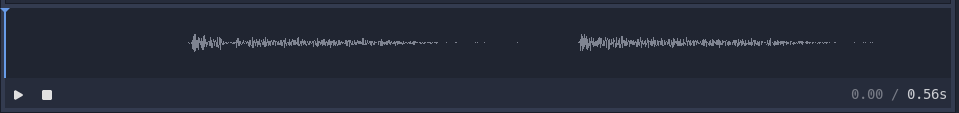
\includegraphics[width=0.9\textwidth]{imagenes/EspectroOndasError.png}
	\caption{Espectro de Ondas del sonido de Error de IGASCE}
	\label{EspectroOndasSonidoError}
\end{figure}


\subsection{Diseño de mecánicas de juego}

% Agregar diagrama de jugabilidad
La condición de victoria en cada nivel implica completar todas las instrucciones proporcionadas por el algoritmo. En los niveles de BFS y DFS, esto implica visitar todos los nodos del grafo. El puntero de instrucciones señala la tarea actual, y el jugador debe ejecutar correctamente lo indicado en la instrucción, ya sea haciendo clic, respondiendo una pregunta, o agregando un nodo a una estructura de datos. Algunas instrucciones, especialmente aquellas que contienen la palabra clave \textit{for}, no requieren acción por parte del jugador. Una vez que se han ejecutado correctamente los pasos requeridos, la instrucción cambiará de color y el cursor se transformará en un ticket.

Para avanzar en las instrucciones, el jugador debe presionar la tecla espacio. Si se presiona la tecla espacio sin completar la instrucción, se activará un sonido de error y el color de la instrucción parpadeará entre rojo y amarillo durante un segundo. Presionar la tecla espacio después de completar la instrucción generará un sonido de confirmación y avanzará a la siguiente instrucción. Si se presiona la tecla espacio cuando no hay más instrucciones, se emitirá un sonido de victoria, permitiendo al jugador pasar al siguiente nivel o visualizar los créditos según corresponda. Este proceso se resume en el diagrama \ref{FlujoMecanicaDeNivel}.

\begin{figure}[h]
	\centering
	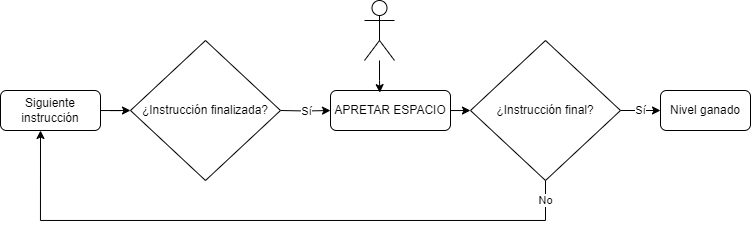
\includegraphics[width=0.9\textwidth]{imagenes/FlujoDeMecanicasDeNivel.drawio.png}
	\caption{Flujo de mecánicas de Nivel. El jugador debe seguir las instrucciones paso a paso.}
	\label{FlujoMecanicaDeNivel}
\end{figure}



\section{Arquitectura de software}

Antes de abordar la arquitectura específica del programa, es crucial comprender cómo se estructuran los programas en Godot. Esta comprensión sirve como base para justificar las decisiones de diseño adoptadas durante el desarrollo de la aplicación.

\subsection{Arquitectura de una aplicación en Godot}

Una aplicación en Godot se construye en base a escenas. Una escena es un conjunto de objetos instanciados al mismo tiempo. Un programa creado en este motor se compone de escenas, que típicamente serán los niveles en un juego. Las escenas tienen un grafo de escena compuesto por uno o más nodos.

Los nodos en Godot son las unidades fundamentales de construcción del programa, representando diversos elementos como botones, texturas, reproductores de sonido o áreas de colisión. Para crear personajes con lógica compleja, como habilidades, movimiento y colisiones, se combinan múltiples nodos.

La estructura del grafo de escena es beneficiosa en el desarrollo de videojuegos, ya que mover el nodo principal de un personaje implica automáticamente el movimiento de elementos asociados, como colisiones, sonidos y texturas. Esto simplifica la manipulación de elementos relacionados.

Otra ventaja clave de Godot es la capacidad de utilizar variables exportadas. Estas variables, cuyos valores se definen desde el editor, permiten instanciar objetos de la misma clase con características distintas \cite{GodotExportVariables}.

En comparación, trabajar a un nivel más bajo con bibliotecas como PyGame, que emplea OpenGL, requiere abordar individualmente cada aspecto de la representación de un objeto. Por ejemplo, mover un personaje implica gestionar texturas y colisiones por separado en el código, aumentando costos y complejidad de desarrollo \cite{GodotCollisionsAndRendering}.

\subsection{Arquitectura de software de la aplicación IGASCE}

La aplicación se desarrolla en diferentes fases, las cuales abarcan tres tipos de escenas: menús, tutoriales y niveles jugables. Cada fase hace uso de módulos distintos, y cada nivel, menú o tutorial representa una escena.

Los menús se construyen principalmente mediante nodos de control, comúnmente utilizados para interfaces gráficas. En este contexto, los menús consisten principalmente en botones que ejecutan códigos específicos según su descripción, dispuestos en formato vertical o en forma de grilla (Ver figura \ref{GodotMenuInterface}).

\begin{figure}[h]
	\centering
	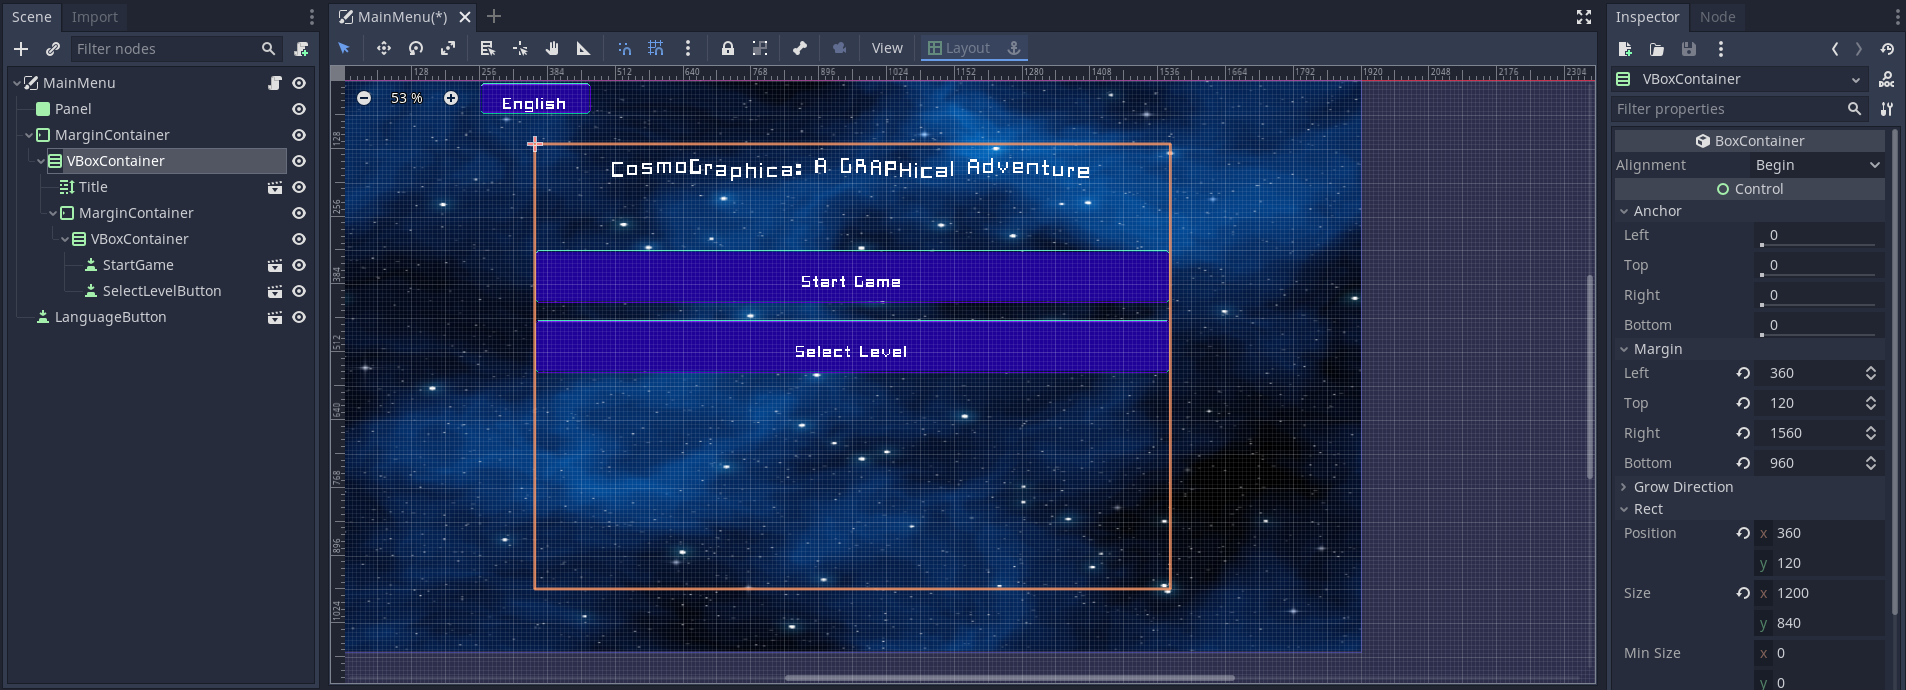
\includegraphics[width=0.9\textwidth]{imagenes/GodotInterfaceMainMenu.png}
	\caption{Interfaz de Godot describiendo la escena del menú principal de IGASCE. El juego públicamente se dio a conocer como CosmoGraphica, pero el proyecto completo se llama IGASCE.}
	\label{GodotMenuInterface}
\end{figure}


Los tutoriales presentan una lógica más compleja y se asemejan a los niveles. A diferencia de las escenas finales, los tutoriales incorporan una ventana de diálogo que busca vincular la historia del videojuego con los elementos interactivos. Además, en los tutoriales, el grafo ya está predefinido, lo que significa que los nodos y arcos ya están establecidos de antemano.

\begin{figure}[h]
	\centering
	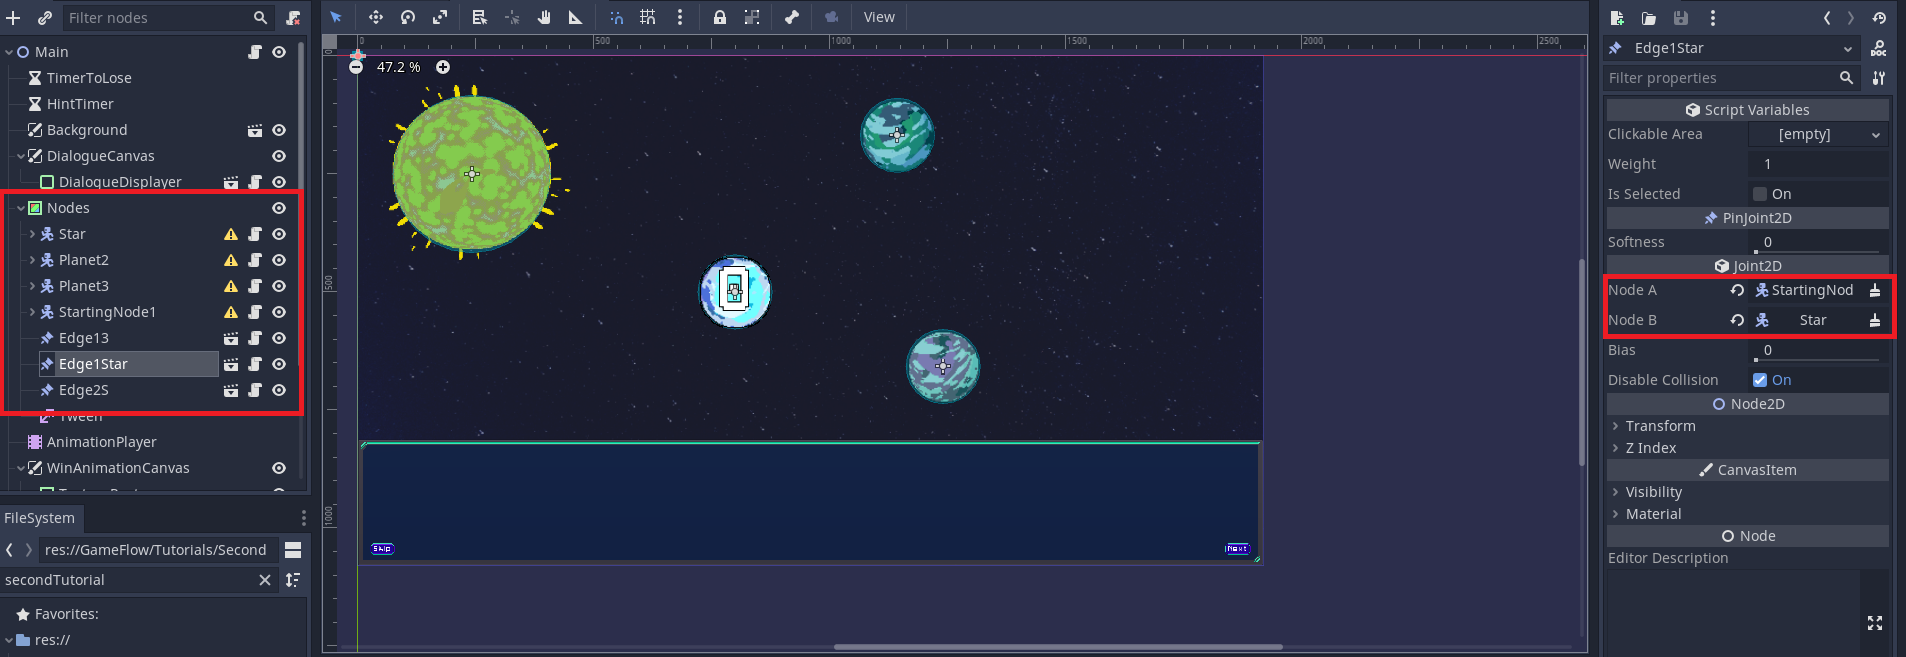
\includegraphics[width=0.9\textwidth]{imagenes/SecondTutorialGraph.png}
	\caption{Interfaz de Godot describiendo el segundo tutorial. En rojo se observa el grafo de escena con los nodos y los arcos ya predefinidos a la izquierda. En la derecha se muestra cómo se unen los arcos, indicando los dos extremos del arco a través de variables exportadas de Godot.}
	\label{SecondTutorialGraph}
\end{figure}


En cuanto a los niveles jugables, hay varios elementos destacables, como el código, las variables, la variable seleccionada y la ventana de juego.

El código que se muestra a la derecha de la pantalla durante el juego está controlado por un nodo de la clase CodeContainer. Este objeto se encarga de recibir la entrada del jugador para avanzar en el código. Si las acciones ejecutadas son correctas, el usuario pasa a la siguiente instrucción, desbloqueando nuevas tareas. La clase CodeContainer posee un arreglo de objetos del tipo CodeLine llamado code\_lines. La clase CodeLine contiene toda la lógica de una única línea de código. Entre sus funciones se encuentran dar énfasis a la línea de código actual, proporcionar feedback al usuario cuando la instrucción de la línea se completa correctamente y verificar constantemente si la instrucción de línea se ha completado correctamente (ver figura \ref{CodeLinesArchitecture}).

\begin{figure}[h]
	\centering
	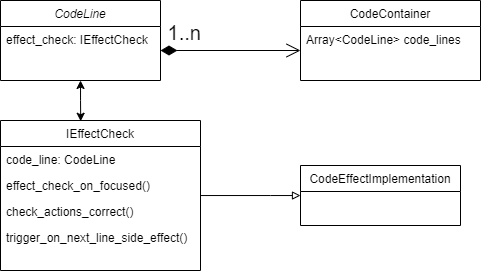
\includegraphics[width=0.9\textwidth]{imagenes/CodeLinesArchitecture.png}
	\caption{Arquitectura de software encargada de la mecánica de ejecución de código dentro del juego.}
	\label{CodeLinesArchitecture}
\end{figure}

Cada CodeLine posee un script que se puede indicar desde el editor de Godot a través de una variable exportada. Este script debe heredar de la clase EffectCheck, la cual actúa como interfaz. Cada script que implemente la interfaz EffectCheck debe definir métodos para: 1) cuando el puntero de instrucción llega a la línea del script; 2) verificar que la instrucción actual se ha realizado correctamente; y 3) si es necesario, manejar efectos colaterales de la instrucción. Este último se utiliza en los ciclos for, donde se mueve el índice utilizado para avanzar por los ciclos y recorrer arreglos, así como para la creación de variables.

En el panel inferior, se encuentran dos clases esenciales: DebugBlock y ADTShower. DebugBlock se encarga de mostrar las variables instanciadas, su nombre y su valor actual. Contiene la lógica para agregar, modificar o eliminar alguna variable. Cada vez que se pasa por un ciclo for o se declara una variable, este ajusta sus variables internas. Hay una variable seleccionada que puede ser manipulada por el usuario de diversas maneras. Al presionar la flecha hacia arriba, se selecciona la variable que está encima de la actual y viceversa para la flecha hacia abajo. En la figura \ref{BFSFullGame}, se observa que la variable ``q'' está seleccionada.

\begin{figure}[h]
	\centering
	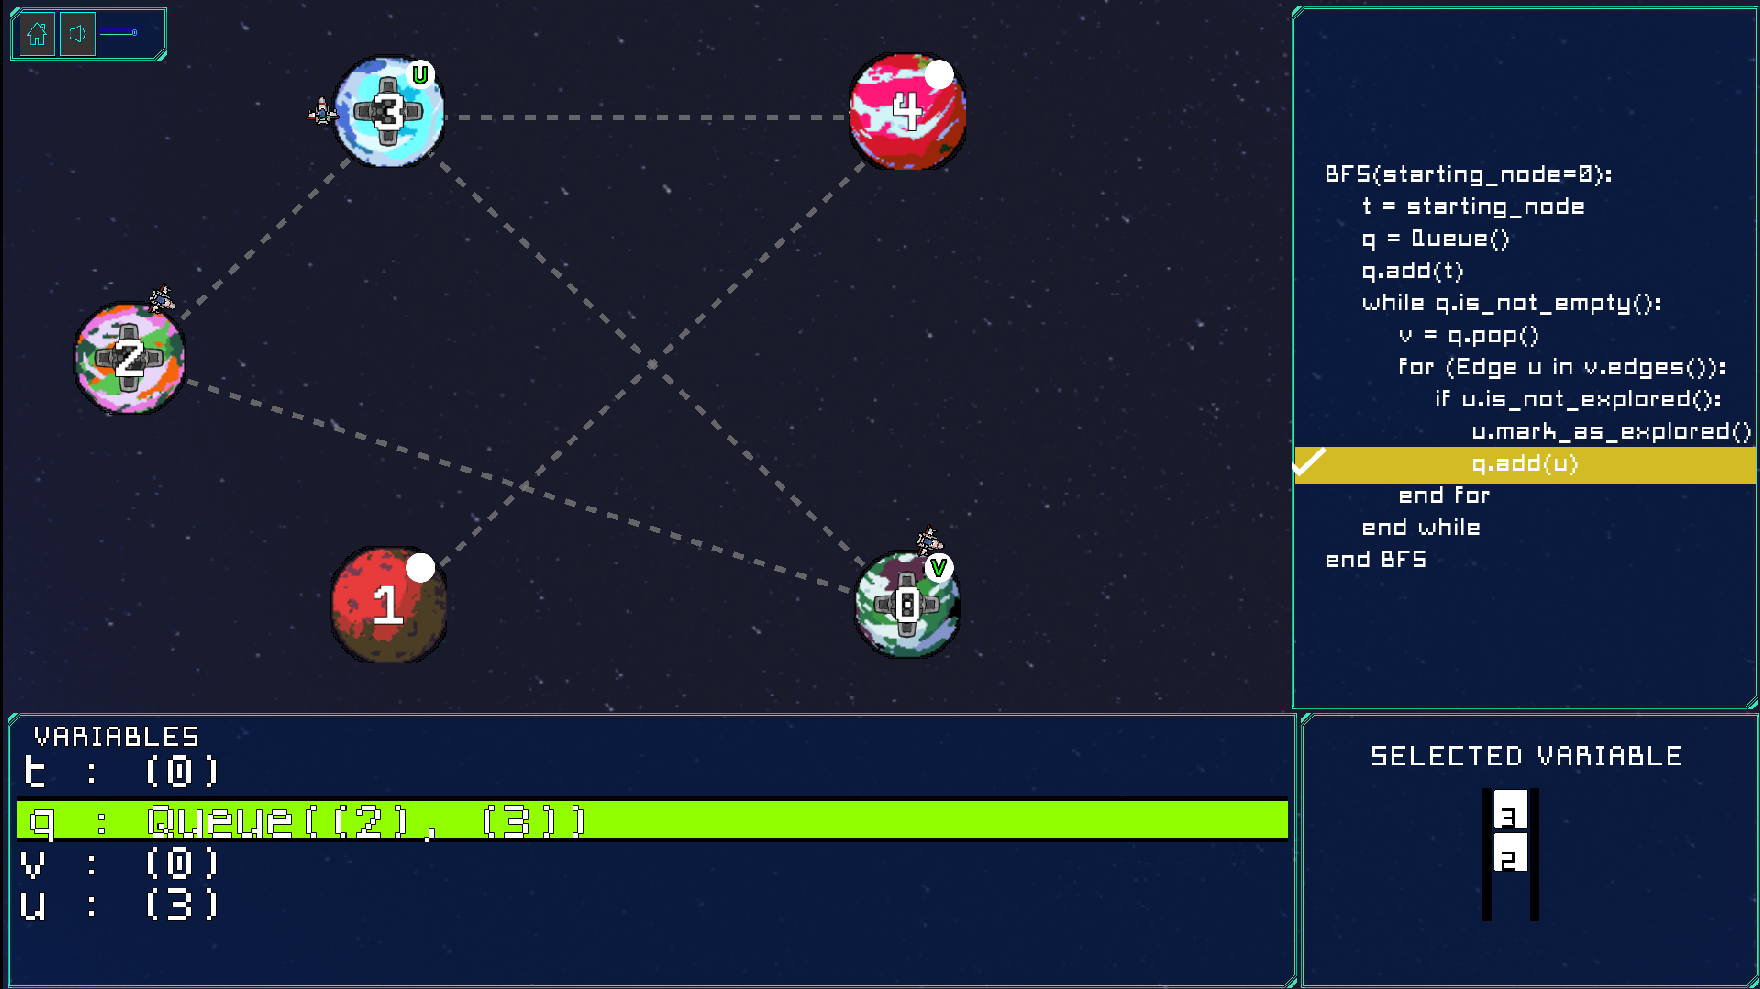
\includegraphics[width=0.9\textwidth]{imagenes/BFSFullGame.png}
	\caption{Nivel jugable BFS. Se observa el código a la derecha, el grafo en el centro, el DebugBlock en la parte inferior izquierda y el ADTShower en la esquina inferior derecha. La varible q está seleccionada.}
	\label{BFSFullGame}
\end{figure}

La clase ADTShower se encarga de mostrar en la esquina inferior derecha la variable que ha sido seleccionada por el usuario. Busca añadir una representación visual al objeto seleccionado para permitir arrastrar nodos a la cola o la pila según el algoritmo que se esté enseñando, BFS o DFS, respectivamente.

Inicialmente, cada cambio en el código debido al efecto de alguna CodeLine o línea de código del juego requería modificar las clases DebugBlock, ADTShower y StoredData (explicada más adelante), además de afectar la misma línea de código. Además, estos efectos deben reflejarse en las líneas de código siguientes para lograr cohesión. Por ejemplo, si la quinta línea crea la variable ``u'' y la sexta la modifica, esto se refleja correctamente en todas las estructuras mencionadas.

Para resolver el problema del alto costo de implementación, se optó por crear una clase llamada ADTMediator, siguiendo el patrón Mediator \cite{Freeman2015TheMP}. Esta clase se inspiró en la arquitectura de React, donde el código generado por React funciona como una única fuente de verdad o "Single Source of Truth" \cite{ReactSingleSourceOfTruth}. Con este tipo de arquitectura, se envía un mensaje a ADTMediator solicitando modificar, crear o eliminar una variable. Esta clase ajusta sus variables internas, luego informa a las clases DebugBlock y ADTShower sobre qué mostrar. Una desventaja de esta arquitectura es que realiza copias innecesarias en cada paso, perdiendo eficiencia. Sin embargo, dado que se trabaja con pocas variables, este costo no es notable a nivel de usuario.


\begin{figure}[h!]
	\centering
	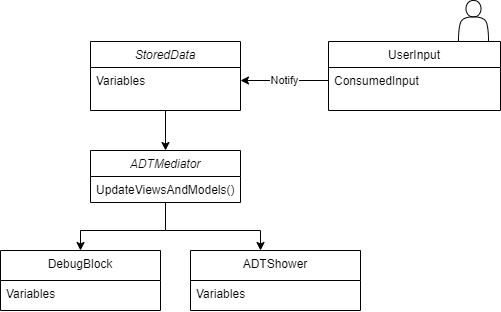
\includegraphics[width=0.9\textwidth]{imagenes/ArquitecturaMediatorAfter.png}
	\caption{Diagrama de un nivel utilizando el ADTMediator, reduciendo el acoplamiento entre clases.}
	\label{ArquitecturaMediatorAfter}
\end{figure}

Una clase que sirve de puente para comunicarse con el ADTMediator es StoredData. Este es un singleton que contiene datos como los avances del usuario en los distintos niveles y el estado del juego. Cuando una línea de código quiere modificar variables dentro del juego, ejecuta un método de este singleton, el cual reenvía esta información al ADTMediator. Esto se hace así porque es fácil obtener el puntero a StoredData, ya que usa el patrón singleton.

Otros singletons son: AudioPlayer, encargado de emitir sonidos específicos en cualquier momento del juego y NotificationManager, que genera ventanas emergentes para el usuario, como menúes, avisos o pestañas donde se debe responder sí o no.
\chapter{Diseño experimental: Metodología}

El propósito de este trabajo fue poner a prueba la hipótesis de que un videojuego educativo puede enseñar algoritmos relacionados con grafos y que puede ser percibido positivamente por parte de los estudiantes.

Para ello, se llevó a cabo un experimento en el que se solicitó a voluntarios que respondieran ciertas preguntas después de probar la aplicación. Este enfoque se considera una metodología simple según \cite{HowGamesComputingEducationEvaluated}, es importante destacar que no es el más adecuado para este tipo de estudios, ya que la mayor validez científica se obtiene con una metodología pre/post/post y un tamaño muestral de 40 individuos o más.

Sin embargo, implementar este tipo de estudios requiere más tiempo por parte de los voluntarios, así como mayores incentivos para su participación y respaldo institucional. Para ejemplificar esto último, la participación en este estudio podría formar parte de una actividad pedagógica en un curso y ser obligatoria.

Se sugieren buenas prácticas metodológicas en \cite{Rogers2002InteractionDesign, MeegaPlusManual, HowGamesComputingEducationEvaluated}, donde se establecen ideas primordiales para identificar las dificultades a resolver. Además, se destaca la importancia de realizar validaciones con tamaños muestrales significativos y representativos del usuario al que está destinado el trabajo. Asimismo, se sugiere aprovechar tecnologías como eye-tracking y telemetría. Sin embargo, la obtención de voluntarios para participar en las pruebas fue un desafío, sobre todo considerando que aquellos que participaran en una prueba inicial no podrían formar parte de las pruebas finales, que se consideraban más relevantes.

Se sugieren buenas prácticas metodológicas en \cite{Rogers2002InteractionDesign, MeegaPlusManual, HowGamesComputingEducationEvaluated}, donde se establecen ideas primordiales para identificar las dificultades a resolver. Además, se destaca la importancia de realizar validaciones con tamaños muestrales significativos y representativos del usuario al que está destinado el trabajo. Asimismo, se sugiere aprovechar tecnologías como eye-tracking y telemetría. Sin embargo, la obtención de voluntarios para participar en las pruebas fue un desafío, sobre todo considerando que aquellos que participaran en una prueba inicial no podrían formar parte de las pruebas finales, que se consideraban más relevantes.


\section{Fases del trabajo de investigación}

El trabajo se dividió en tres fases, las cuales constan de distintas preguntas después de probar la aplicación.


\subsection{Fase exploratoria}

En esta primera fase, el objetivo fue recopilar retroalimentación y opiniones de usuarios de manera abierta, utilizando metodologías de pensamiento en voz alta con personas experimentadas en grafos. Se optó por esta metodología por dos razones. En primer lugar, si un usuario conoce el algoritmo y la estructura de datos pero no comprende el videojuego, entonces existen problemas de usabilidad, justificando el enfoque inicial con personas expertas.

En segundo lugar, los usuarios expertos tienden a expresarse de manera más natural cuando pueden emitir opiniones en el momento, por lo que se prefirió evitar encuestas o escalas posteriores a la experiencia. Resulta crucial que los expertos expresen sus impresiones a medida que los elementos del videojuego aparecen en pantalla y no después de la experiencia, para comprender mejor lo experimentado al usar la aplicación por primera vez. Hay animaciones que deben captar la atención en el momento, como la pista visual del ratón indicando al usuario que haga clic izquierdo en un planeta.

Este desarrollo fue iterativo. Primero se hacían cambios a la aplicación basados en los últimos comentarios recibidos. Luego, se le mostraba la aplicación a usuarios expertos, estos daban su opinión y se volvían a aplicar los cambios. Este proceso se hizo 8 veces con el curso ``CC7970 - Trabajo de Tesis I''.


\subsection{Fase de evaluación académica y percepción de usuario}

En esta fase, se logró la participación completa de una muestra de 15 personas, a quienes se les ofreció un incentivo monetario para evitar sesgos asociados a la voluntariedad y para aumentar la participación \cite{Marinescu2018IncentivesCR, Dallmeyer2023ToPayOrNot}.

Para iniciar esta etapa, se realizó una convocatoria voluntaria en el foro de las tres secciones de Algoritmos y Estructuras de Datos de la Universidad de Chile durante las primeras dos semanas del semestre de primavera del año 2023. Se ofreció una remuneración a todas las personas que completaran la experiencia, la cual tenía una duración promedio de 45 minutos. 

Las personas que rinden este curso suelen estar en su quinto semestre de la carrera, aunque algunas también lo rinden de forma más tardía en sus carreras, sobre todo cuando son de otras especialidades como Ingeniería Eléctrica o Industrial. Estos suelen tener nociones de programación, como declaración de variables y control de flujo, pero no necesariamente sobre estructuras de datos. Estos estudiantes rondan los 21 a 23  años de edad.

La convocatoria se realizó por dos medios. Por una parte, se escribió un mensaje en la comunidad de Telegram invitando a la gente del curso a participar del estudio, y por otra parte, el equipo docente de cada sección del curso CC3001 - Algoritmos y Estructuras de Datos, escribió un mensaje en el foro invitando a sus estudiantes a participar.


La experiencia constaba de tres partes: realizar la prueba de usuario, completar un formulario que utilizaba la escala de Likert basado en el modelo MEEGA+ \cite{meegaplus}, y responder a una prueba escrita basada en exámenes previos del curso CC3001 antes mencionado.

El modelo sistemático MEEGA+ \cite{meegaplus} está diseñado para evaluar videojuegos educativos, buscando evaluar la percepción de la calidad de un videojuego desde la perspectiva del estudiante en el contexto de la enseñanza de la computación. El formulario utilizado en este estudio, basado en MEEGA+, se encuentra en el anexo A.

La medición del rendimiento académico se lleva a cabo mediante una prueba escrita con dos preguntas, basadas en una pregunta de un examen del ramo de Algoritmos y Estructuras de Datos de la misma facultad. La prueba escrita se encuentra en el anexo anexo B.


\subsection{Encuesta libre}

% Anotar aquí antes de que termine la tesis cuánta gente fue en total.

Con el objetivo de ampliar el estudio y aumentar el tamaño de la muestra, se llevó a cabo una tercera experiencia abierta al público en general con conocimientos en programación. Se emitió una invitación en diversas comunidades de videojuegos para probar el juego educativo y completar el formulario. Dado que las experiencias podían variar significativamente, se incorporó una pregunta sobre el nivel de experiencia en programación para permitir la segmentación. El formulario utilizado también se basó en el modelo MEEGA+, pero las respuestas recolectadas se almacenaron en una base de datos separada del grupo anterior. Aquí se mostraron dos versiones, una en español y otra en inglés para aumentar el tamaño de la muestra. En total, 12 personas participaron de esta experiencia.

\chapter{Resultados}

\subsection{Prueba académica}

Las 15 personas que hicieron la prueba tuvieron ambas respuestas correctas, identificando correctamente el recorrido BFS y DFS en cada caso.


\subsection{Formulario MEEGA+: Percepción de usuario}

% Hablar de la suma de puntaje y puntaje promedio para los dos casos: De fase exploratoria y fase posterior.
Las respuestas al formulario se encuentran en: \href{https://docs.google.com/spreadsheets/d/1DlxUT5o-nRknYXGtFWqkXX2ZkuEZJZsow4DbW6bUTh8/edit?usp=sharing}{https://docs.google.com/spreadsheets/d/1DlxUT5o-nRknYXGtFWqkXX2ZkuEZJZsow4DbW6bUTh8/edit?usp=sharing}


Debería poner aquí los gráficos o en un anexo?
% Poner acá gráficos y demás


\chapter{Discusión}

% \cite{Yu2020TheEffectsOfEducationGames} Difficulty in Determining the Effectiveness of Educational Games
% Mencionar aquí que desde ya se ven varias debilidades en general en el área STEM, además que no es aceptado.
% Suggestions for Educational Game Designers
% While many studies have been committed to the effect of educational games on
% learning, few of them have shed light on their design (Fanfarelli, 2020). Game
% features, e.g. perceived usefulness, ease of use, and goal clarity, could increase
% student engagement and improve the enjoyment of games, which should be
% stressed by game designers (Y. C. Wang et al., 2017). 
% Indicar que este videojuego no fue hecho por un diseñador o fue pensado fuertemente en su diseño
% Y que se hizo énfasis en la metolodogía de: línea de código o instrucción con un correlato de acción por parte del jugador
% en el videojuego.


\section{Fortalezas de la metodología aplicada}

La principal fortaleza de la metodología empleada radica en la utilización de un formulario estandarizado y previamente validado. Se tiene una alta confianza en que dicho formulario mide de manera efectiva lo que busca evaluar, como se validó a través de la alfa $\alpha$ de Cronbach, medida en el trabajo de Petri et al. \cite{MeegaPlusManual}. Esta medida indica que las preguntas evalúan efectivamente lo que el cuestionario buscan evaluar \cite{MeegaPlusManual}. Esta metodología proporciona una valoración numérica de la calidad del juego según las opiniones de los usuarios, representando este valor numérico como un rasgo latente (latent trait) comúnmente denotado como $\theta$ en IRT \cite{maldonado2021statistical, RashMeasurementTheoryAndrichMarais}.

El proceso de diseño se considera robusto, ya que incorporó retroalimentación de expertos y la aplicación de la metodología de ``Loud Thinking'' en cada iteración. Esto permitió que los jugadores se familiarizaran adecuadamente con el juego, culminando en la exitosa realización de la prueba escrita. Se ha comprobado empíricamente cómo la usabilidad mejoró en cada fase del desarrollo.

Además, el proceso está rigurosamente documentado, ya que la historia completa del desarrollo se encuentra disponible en un repositorio de Github \cite{GithubRepo}. Esto posibilita que cada iteración del juego sea reproducible, incluso los experimentos con usuarios, lo que permite a otros investigadores volver a versiones anteriores del videojuego y realizar pruebas con diferentes grupos de usuarios en cada instancia.

\section{Debilidades y mejoras para la metodología aplicada}

Una debilidad identificada es que la prueba académica no logró detectar diferencias entre los grupos, asignando un puntaje perfecto a todos los estudiantes. Se proponen dos metodologías para mejorar la precisión de los resultados:

1) Aplicar A/B testing: comparar la metodología del videojuego educativo con otra aplicación o la lectura de un artículo relacionado con la misma materia que busca enseñar el videojuego. Luego, evaluar a los estudiantes con un examen escrito más extenso para establecer una graduación y realizar una comparación directa entre distintos métodos de educación.

2) Tomar una muestra aleatoria de estudiantes: Idealmente seleccionar personas que estén cursando Algoritmos y Estructuras de Datos y mostrarles el videojuego. Posteriormente, realizar un examen y medir las diferencias entre el grupo que probó el videojuego y el grupo que no lo hizo. Sin embargo, esto requiere apoyo institucional y garantizar la inclusión de la materia de grafos en el curso.

Un aspecto a mejorar es que el videojuego no tiene componentes sociales, tales como multijugador, ya sea de forma competitiva o cooperativa. Estos elementos se descartaron debido a la dificultad para aplicar pruebas de usuario multijugador y la complejidad de agregar cooperatividad o competitividad a nivel de diseño. El modelo MEEGA+ \cite{meegaplus} busca evaluar también esta dimensión social. Para objeto de la evaluación de la calidad de juego, las preguntas relacionadas con este item se omitieron en el formulario.

Por otra parte, no se puede garantizar la heterogeneidad de la muestra. Existe el sesgo del voluntario, que afecta según \cite{volunterBias}. El caso ideal implica una separación aleatoria en los cursos como parte de las actividades de la clase. No obstante, es probable que aún existan sesgos en los cursos debido a la selección de estudiantes de carreras asociadas a computación o informática. Se recomienda acotar el grupo solo a estudiantes afines a la informática. Por esta misma razón, también se aconseja acotar estos estudios únicamente a estudiantes de carreras relacionadas con STEM y agregar segmentación.

%  Por otra parte, existe el sesgo de novedad. % CITAR
Además, según libros como \cite{Rogers2002InteractionDesign}, es más efectivo realizar una prueba dos semanas después para medir aprendizajes efectivos. No obstante, esto fue difícil de realizar dadas las condiciones del trabajo, ya que conseguir voluntarios en un contexto donde los estudiantes prefieren dedicar su tiempo a preparar exámenes en lugar de participar en una actividad universitaria fue un desafío. Se sugiere buscar apoyo institucional y aumentar los incentivos a la participación, por ejemplo, mediante actividades que fomenten la comunidad al inicio del semestre académico.

Finalmente, el autor de este trabajo no es un diseñador de videojuegos y su principal énfasis está en la programación. Se destaca el rol y la importancia del diseño en los videojuegos, que deben ser atractivos y ofrecer mecánicas que recompensen al jugador, así como agregarle una dimensión social a través de un ranking, componentes cooperativas o competitivas. La narrativa tampoco está completamente desarrollada; no presenta una historia con un fin, desarrollo de personaje ni antagonista. Estos elementos suelen despertar más el interés del jugador \cite{Zea2014ModelingST, FrangoSilveira2019BuildingEN}.


\section{Trabajo futuro}

% Poner aquí ideas locas que había comenzado a anotar con Jeremy 
% Quizás debería poner eye tracking en el marco teórico?
% Quizás también poner elementos de los videojuegos en el marco teórico, como sonidos, interfaces, controles, tiempos, mecánicas.


En el futuro, esta aplicación o sus derivaciones podrían evaluarse en otros contextos, con muestras más extensas, para garantizar una validez estadística más sólida. Se recomienda la implementación de un diseño experimental que mitigue sesgos como el factor de novedad y el sesgo del voluntario. Además, se sugiere medir los resultados del aprendizaje en distintos intervalos temporales al utilizar esta aplicación. Considerando que la aplicación fue concebida como un complemento a la enseñanza tradicional y para ser utilizada en pausas activas, se propone estudiarla en grupos donde se haya empleado como herramienta complementaria y comparar los resultados con otro grupo que no la haya utilizado.

Una mejora en la recolección de datos sería la aplicación de principios de telemetría y el uso de tecnologías adicionales que profundicen en el estudio de usabilidad y experiencia del usuario. Existen frameworks que sirven como servidor para aplicaciones relacionadas con videojuegos y que ofrecen servicios de telemetría y análisis de datos, como PlayFab \cite{PlayFabTelemetry}. Tecnologías como eye-tracking o biofeedback podrían proporcionar una comprensión más detallada y estandarizada de la experiencia de los usuarios con el videojuego, identificando áreas de mejora \cite{Zain2011EyeTI}. Por ejemplo, se espera que los usuarios visualicen el código cada vez que realizan un paso, y esto podría confirmarse mediante eye-tracking. En el trabajo de \cite{Zain2011EyeTI}, se observa cómo los usuarios interactúan con las interfaces en un videojuego educativo.

Una posible expansión de este trabajo implica la exploración de otras estructuras de datos y algoritmos que no necesariamente estén vinculados a los grafos. El software desarrollado está diseñado para ser adaptable a otros algoritmos, aunque requeriría trabajo adicional para determinar visualizaciones, representaciones y mecánicas específicas para cada uno.

Desde la perspectiva del diseño de juegos, se podrían agregar más elementos de gamificación, como la adquisición de nuevos elementos, desbloqueo de mecánicas, acumulación de puntos, establecimiento de un ranking global, sistema de logros y finales alternativos.
% TODO BUSCAR CITA
\chapter{Conclusión}

El videojuego logra su objetivo de enseñar los algoritmos de BFS y DFS, como evidencian los resultados obtenidos por estudiantes de informática de la Universidad de Chile. Estos estudiantes demostraron comprender los algoritmos, así como la naturaleza de los grafos, al responder de manera acertada a una prueba asociada al juego.

Por otra parte, el juego ha recibido una evaluación positiva y se considera, según el modelo MEEGA+ \cite{meegaplus}, como un juego de calidad. A pesar de las mejoras identificadas durante el proceso, el juego ha sido bien recibido por los estudiantes, y su percepción positiva puede influir beneficiosamente en la motivación y, por ende, en los resultados académicos.

Las hipótesis son verdaderas. La primera hipótesis indica que un videojuego que enseña sobre grafos puede enseñar a los estudiantes sobre los algoritmos BFS y DFS. La segunda hipótesis, \emph{H2 Un videojuego que enseñe grafos será percibido de manera positiva por los estudiantes que todavía no aprenden sobre esos contenidos}, también es correcta, medida a través del valor $\theta$ entregado por el modelo MEEGA+.

Este trabajo sienta bases para futuras investigaciones, especialmente en relación con el diseño de videojuegos educativos y su impacto en la educación en informática. La metodología utilizada aquí puede ser perfeccionada en trabajos futuros para evaluar mejor la comprensión de los conceptos enseñados mediante este enfoque lúdico.

Para casos futuros, se recomienda emplear una metodología de estudio pre/post/post como se indica en \cite{HowGamesComputingEducationEvaluated}, aumentar el tamaño muestral y utilizar al menos dos grupos: uno de control y otro de tratamiento para medir mejor las diferencias. 



% Énfasis en Resultados Positivos: Resalta de manera más específica los resultados positivos obtenidos, como el hecho de que los estudiantes lograron comprender los algoritmos y la estructura de los grafos, así como aprobar la prueba asociada. Esto ayuda a consolidar la efectividad del videojuego como herramienta educativa.

% Impacto en la Motivación: Puedes profundizar en cómo la percepción positiva del juego podría influir en la motivación de los estudiantes. ¿Se notó un aumento en el interés por el tema? ¿Hubo comentarios que sugieran un cambio en la actitud hacia el aprendizaje?

% Relación con Otros Métodos de Enseñanza: Considera mencionar cómo este enfoque se integra o complementa con otros métodos de enseñanza tradicionales. ¿El juego podría servir como apoyo en determinadas etapas del aprendizaje?

% Desafíos y Lecciones Aprendidas: Brevemente, comparte los desafíos encontrados durante el desarrollo e implementación del videojuego, así como las lecciones aprendidas. Esto podría incluir aspectos técnicos, metodológicos o de diseño que podrían ser útiles para otros investigadores o desarrolladores en proyectos similares.

% Relevancia en la Educación Actual: Haz hincapié en la relevancia del juego en el contexto educativo actual. ¿Cómo se alinea con las tendencias y necesidades de la educación en informática?

% Posibles Extensiones del Trabajo: Además de lo que ya has mencionado sobre futuras investigaciones, podrías sugerir posibles extensiones o mejoras específicas para el juego en función de los comentarios y resultados obtenidos.

% ver https://www.overleaf.com/learn/latex/Glossaries
% \input{glosario.tex} % opcional

\nocite{*}
\bibliographystyle{plain}
\bibliography{bibliografia}

% opcional ...
% \begin{appendices}w
\chapter{Anexo}



\chapter*{Anexo B: Prueba de conocimiento de grafos} \label{AnexoB}
\textbf{Test para verificar aprendizaje de BFS y DFS}

Considere el siguiente grafo:

\begin{figure}[h]
        \centering
    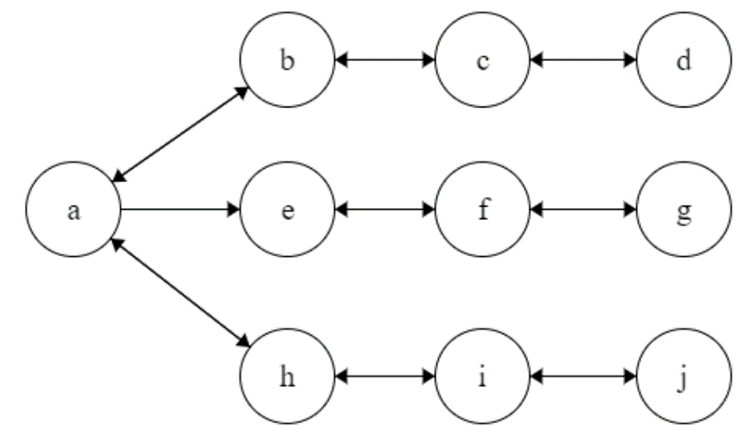
\includegraphics[width=0.6\textwidth]{imagenes/GrafoPrueba.png}
\end{figure}

Muestre el recorrido de un grafo desde el nodo a utilizando distintos los dos algoritmos de búsqueda vistos. \textbf{Agregue una numeración al lado de sus arcos para indicar el orden} en que se explorando.
Por ejemplo, en el siguiente grafo, si se recorre \textbf{a}, \textbf{b} y \textbf{c} partiendo desde \textbf{a, pasando por b y llegando a c}, el resultado esperado es el siguiente:

\begin{figure}[h]
        \centering
        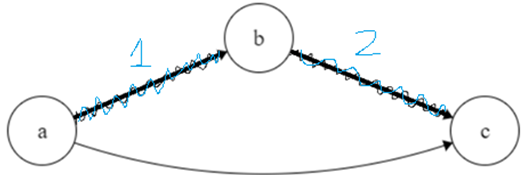
\includegraphics[ width=0.5\textwidth]{imagenes/GrafoPruebaEjemplo.png}
\end{figure}

\newpage 
1.	Aplique el algoritmo \textbf{Búsqueda en Profundidad (DFS / Depth First Search)} para mostrar cómo se recorre un grafo partiendo desde el nodo a.

\begin{figure}[htbp]
        \centering
    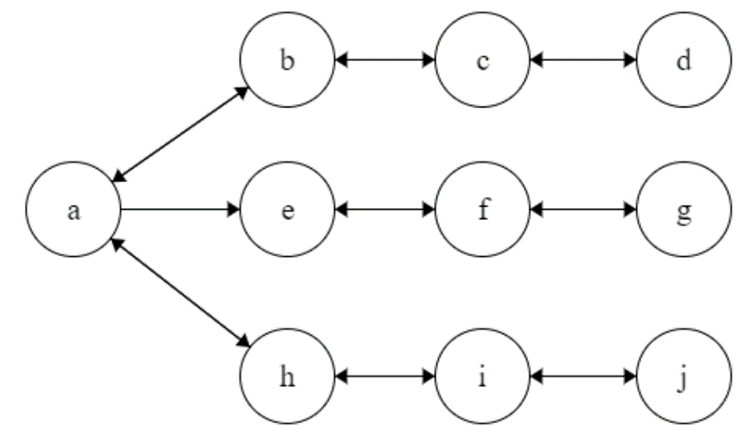
\includegraphics[width=0.7\textwidth]{imagenes/GrafoPrueba.png}
\end{figure}

2.	Repita lo anterior usando el algoritmo de \textbf{Búsqueda en Achura (BFS / Breadth First Search)}

\begin{figure}[htbp]
        \centering
    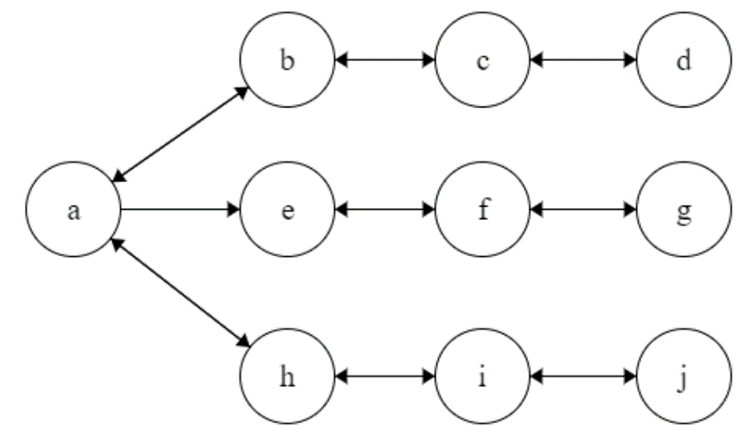
\includegraphics[width=0.7\textwidth]{imagenes/GrafoPrueba.png}
\end{figure}

%\newgeometry{margin=0.1in}
%\begin{figure}[htbp]
    %    \centering
    %    \fbox{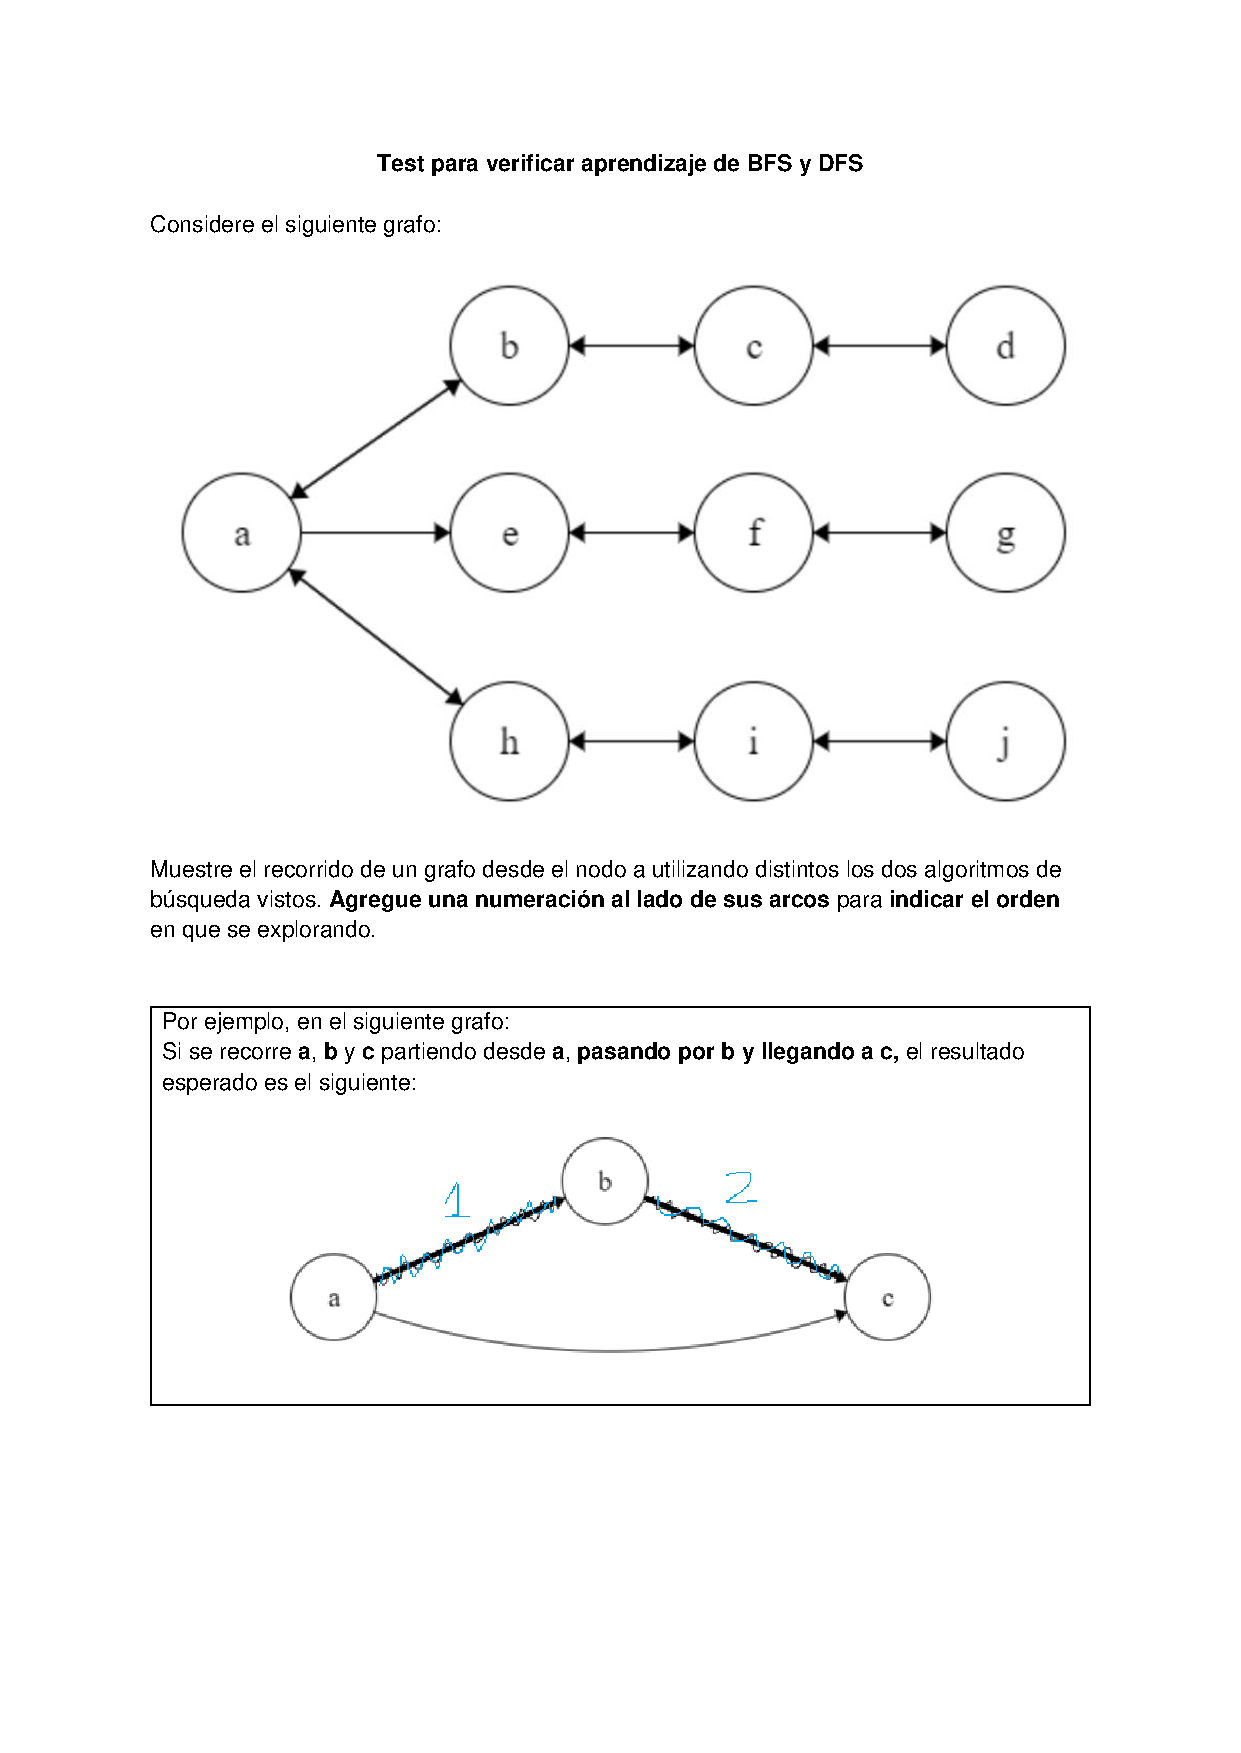
\includegraphics[page=1, width=0.7\textwidth]{imagenes/TestParaVerificarAprendizaje.pdf}}
    %    \caption{Your caption here}
    %    \label{fig:yourlabel}
    %\end{figure}
%\restoregeometry

\chapter{Anexo C: Respuestas de pruebas de usuario}\label{AnexoC}



\chapter*{Anexo D: Aprobación de Comité de Ética}\label{AnexoD}
% Poner aquí el PDF del comité de ética

Revisar siguiente página. Esta aprobación se dio como respuesta a una solicitud para realizar un trabajo de título con personas, para asegurarse que se enmarcara dentro del marco ético establecido por la facultad.

\newgeometry{margin=0.0in} % Eliminamos bordes temporalmente

% Páginas 1 y 2 en dstintas páginas
\begin{figure}[h]
   \centering
   \fbox{
\includegraphics[page=1, width=0.9\textwidth]{imagenes/ComiteEticaFirmado.pdf}}
\end{figure}

\begin{figure}[h]
   \centering
   \fbox{
\includegraphics[page=2, width=0.9\textwidth]{imagenes/ComiteEticaFirmado.pdf}}
\end{figure}

\restoregeometry

\chapter*{Anexo E: Consentimiento de participación voluntaria}\label{AnexoE}

Revisar siguiente página. Este consentimiento debió firmarlo cada participante antes de empezar con la actividad. Era requerido por parte de la facultad para asegurar que cada individuo voluntario estuviera de acuerdo con formar parte del trabajo.

\newgeometry{margin=0.0in}

\begin{figure}[h]
   \centering
   \fbox{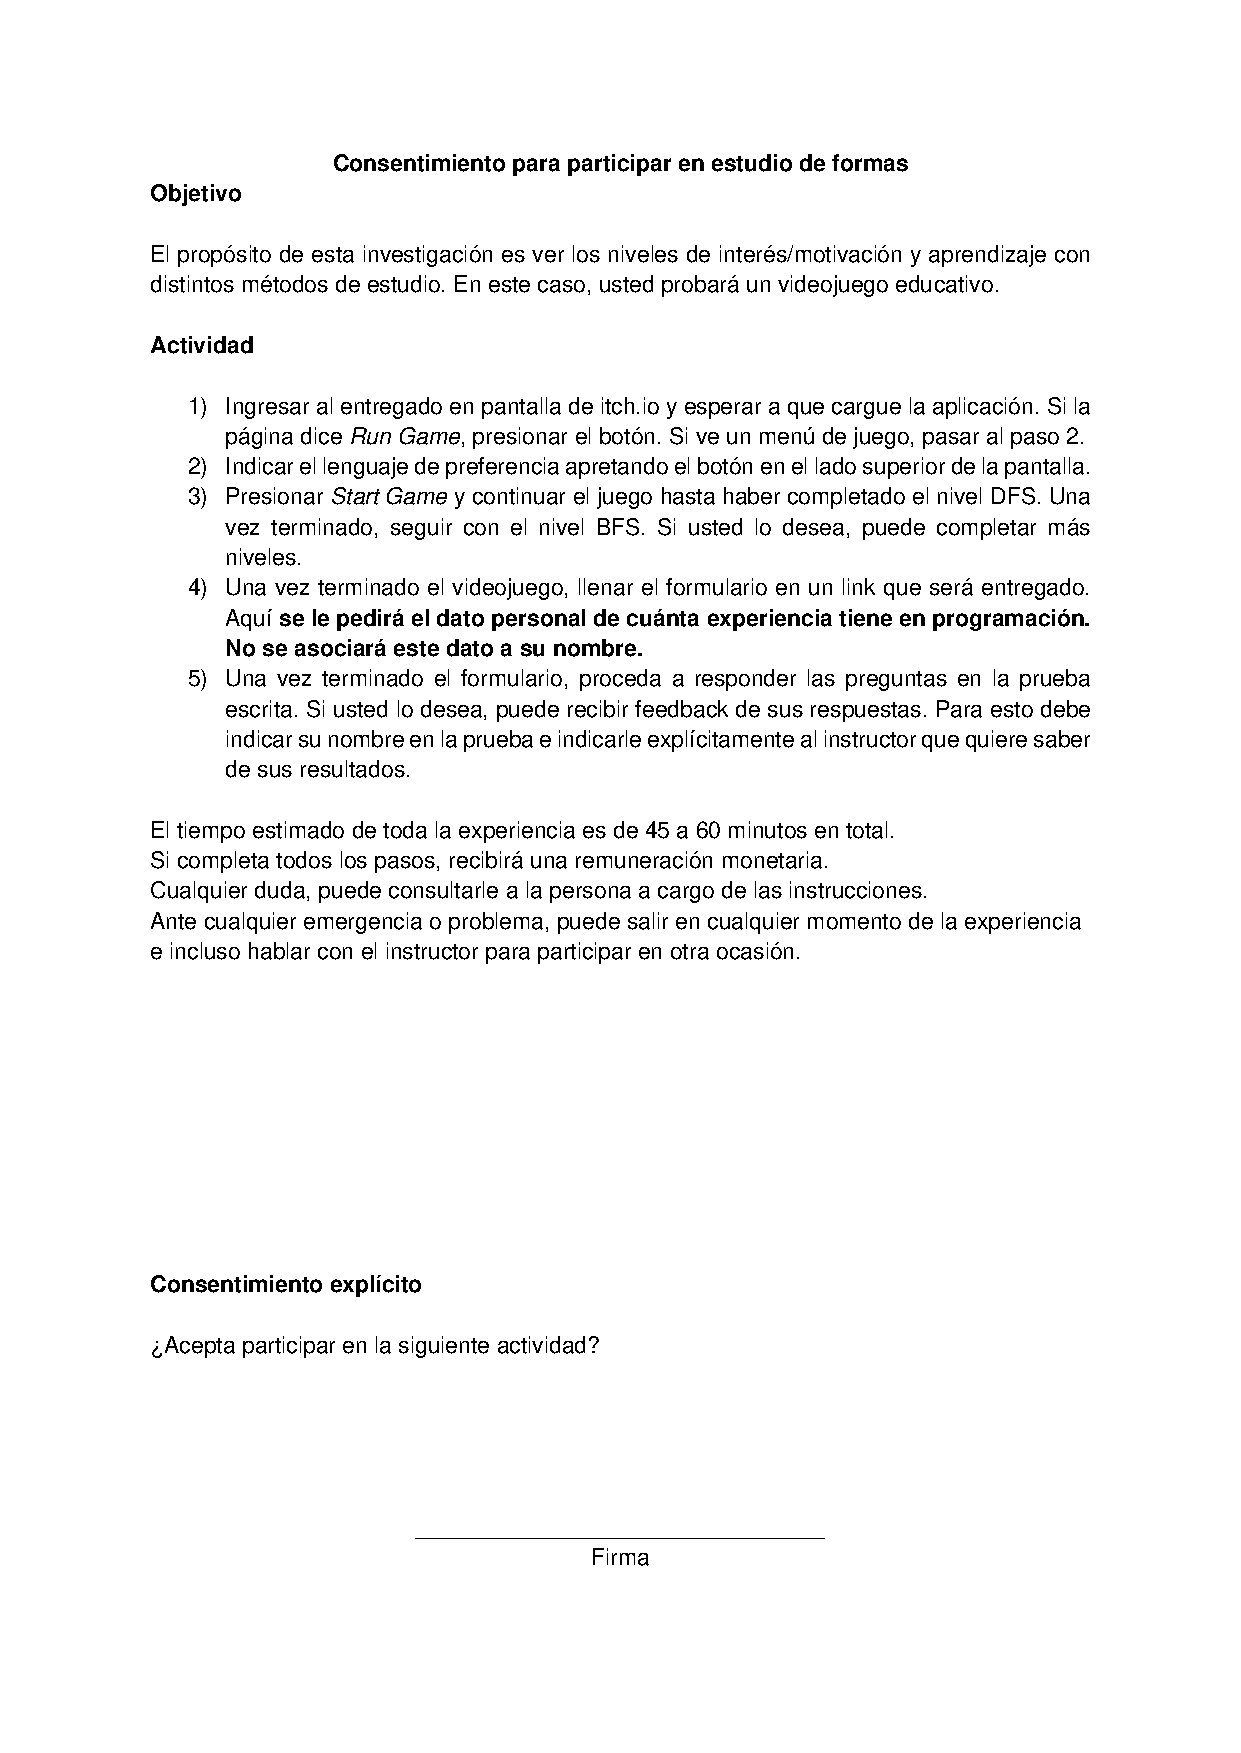
\includegraphics[page=1, width=0.9\textwidth]{imagenes/ConsentimientoInformadoCosmoGraphica.pdf}}
\end{figure}

\restoregeometry
\chapter*{Anexo F: Comentarios abiertos entregados por los voluntarios}\label{AnexoF}

\newgeometry{margin=0.5in}

% 1.1
Las siguientes tablas de comentarios muestran las respuestas del primer grupo, aquel que realizó la prueba académica.

\begin{table}[h]
   \centering
   \caption*{\textit{Comentarios del grupo que realizó la prueba académica frente a la pregunta: Nombra aspectos fuertes del juego}}
   \begin{tabular}{|p{\linewidth}|}
   \hline
   \textbf{Comentario} \\\hline
   Es una forma distinta de aprender. Es interactivo. Me gusta que sea de prueba y error. \\\hline
   Enseña de manera correcta el algoritmo \\\hline
   Era intuitivo y fácil de entender \\\hline
   El aspecto que me llamó mucho la atención y lo destaco como un aspecto fuerte del juego, fue la forma interactiva de mostrar un código de programación y conceptos detrás de estos mismos. \\\hline
   
   De esa forma, se puede visualizar de mejor manera la dinámica detrás de un algoritmo (que muchas veces eso llega a ser un problema a la hora de analizar su funcionamiento, en especial si son algoritmos más complejos) \\\hline
   Me parece que al ser interactivo se entienden mejor los conceptos, además los movimientos de la nave ayudan a entender gráficamente cómo funciona el algoritmo \\\hline
   El diseño y la historia planteada son atractivos, como también la jugabilidad, es idónea para adquirir habilidades de programación. \\\hline
   
   Es intuitivo y no tan difícil de entender la idea, el diseño de niveles y la interfaz de usuario \\\hline
   Incorporar animales tiernos y buena música aporta mucho a la satisfacción y motivación de terminar los niveles \\\hline
   El acompañamiento visual de las líneas del código ayuda mucho al entendimiento del algoritmo sin tener la necesidad de explicar textualmente la función de cada uno \\\hline
 Me gustó poder saltarme las instrucciones porque no me gusta leerlas, menos si es un juego. Me gustaron los colores, llama la atención a pesar de ser un juego sin mucho detalle \\\hline
    La atmósfera del juego permite conectar fácilmente con la experiencia de aprendizaje, además su temática me parece bastante atractiva \\\hline
    Es entretenido y super fácil de seguir las instrucciones \\\hline
    Me gustó que agregue una imagen sobre el contenido de programación que se tratará en cada nivel, eso me facilita el aprendizaje y la idea de lo que estoy realizando. Además, el juego ayuda bastante si te equivocas o no realizaste una acción (como seleccionar el nodo u otros) \\\hline
    Es interesante que sea de programación y astronomía/ es desafiante \\\hline
    Es un juego entretenido, los gráficos llaman la atención, interactivo y uno puede quedarse pegado jugando \\\hline
    Las gráficas son muy bonitas y atractivas, invitan a jugar  \\
   \hline
   \end{tabular}
\end{table}

\restoregeometry

% 1.2

\newgeometry{margin=0.5in}
\begin{table}[h]
   \centering
   \caption*{\textit{Comentarios a la pregunta ``indica una o más sugerencias para mejorar el juego''. Grupo que realizó la prueba académica.}}
   \begin{tabular}{|p{\linewidth}|}
   \hline
   \textbf{Comentario} \\\hline
   Mejorar colocación de títulos. \\ \hline
   Hacerlo menos tedioso, quizás agregar alguna música acorde, poner el código de manera más amigable en vez de un código tan seco, que el grafo inicial sea más pequeño; \\ \hline
   Quizás se podría explicar un poco más de qué significa el código de la derecha para gente que no tiene ni idea de programación. Que es un for, un while y demás, explicar cómo se recorre y por qué; \\ \hline
   Agregar muchos más niveles que formen una gran escalera progresiva de contenidos a aprender. También podría sugerir que en el momento que la persona no interactúe con el juego en un tal momento del algoritmo, el juego diga mini hints que ayuden a pensar a la persona de lo que debería hacer en donde está estancado. Tal vez que sea más largo o que tenga más ejercicios por algoritmo; \\ \hline
   La tipografía de la letra y los colores para facilitar la lectura, hay números que se confunden con letras y requieren contraste con el resto del juego, un buen ejemplo de esto sería el final fantasy donde el texto es solamente un fondo negro con letras blancas los controles, al momento de agregar los planetas yo pensaba que era apretar r no más pero había que poner el mouse sobre el planeta cambiar la letra no me gustaba; \\ \hline
   Las palabras del texto explicativo deberían resaltar las instrucciones centrales. \\ \hline
   Sería positivo incorporar un botón de ayuda, en algunas partes sentí que me quedé atrapado.; \\ \hline
   Las instrucciones del principio deberían ser entregadas de una manera más simple y directa. Quizás un cuadro con una lista de todo lo que hay que hacer al inicio podría ayudar.; \\ \hline
   Mejorar la fuente de texto, se me complicó en ciertos casos leer algunas letras.; \\ \hline
   Podría ser la música que era un poco desesperante y se podría hacer un pequeño tutorial explicando las funciones que se utilizan; \\ \hline
   Si el juego busca enseñar programación, sería bueno colocar un módulo donde se pueda explicar mejor el código o dar alguna explicación de ciertas funciones que no sabía qué hacían pero igual tenía que apretar espacio para pasarlas (podría ser una pequeña explicación al pasar el mouse por sobre el texto). Quizás no era de importancia para el juego, pero como no conozco mucho el lenguaje con el que se utilizó e igual sé programar, sería interesante poder conocer qué significan tales funciones.; \\ \hline
   Encuentro que el juego se puede completar sin entender del todo la diferencia entre queues y stacks, solo mecanizando el seguir las instrucciones del panel derecho. Ambos niveles se diferencian en que el primero es mucho más rápido de recorrer y mecanizar, mientras que el segundo plantea más dificultad, pero no queda completamente claro en cuál se usan queues y en cuál stacks.; \\ \hline
   Quizás faltaron planetas para que se notara más el hecho de acumular elementos en queues o stacks y la forma en que estos se extraen, o quizás sería más sencillo entender estos conceptos si el juego solo consistiera en clickear planetas para ir recorriendo los mapas, sin necesidad de apretar teclas como espacio, R, W o S, ya que a la larga esta mecánica distrae un poco de entender realmente cómo están operando los algoritmos. \\ \hline
   \end{tabular}
\end{table}

\restoregeometry

% 1.3
\newgeometry{margin=0.5in}
\begin{table}[h]
   \centering
   \caption*{\textit{Comentarios a la pregunta ``Algún otro comentario?''. Grupo que realizó la prueba académica.}}
   \begin{tabular}{|p{\linewidth}|}
   \hline
   \textbf{Comentario} \\\hline
   Muy buen juego, es a mi gusta una forma divertida de aprender a manejar grafos. \\ \hline
   Muy entretenido, viva los pandas rojos!! \\ \hline
   Muy interesante y entretenida la propuesta de este juego. Espero que se logré desarrollar más y más :3 \\ \hline
   No soy fan del tema espacial pero si me gusto el juego \\ \hline
   muy bueno \\ \hline
   Las palabras del texto explicativo deberían resaltar las instrucciones centrales. \\ \hline
   Hay unos pasos en los que no hay que hacer ninguna acción, por ejemplo el comando s.pop, y al principio eso me confundió un poco por no tener la certeza de cuál era su función dentro el algoritmo. Creo que eso es parte del desafío del juego y se logra comprender gracias al acompañamiento visual y sonoro \\ \hline
   creo que a pesar de ser estudiante de ingeniería  tengo poca noción de la programación, así que para mi al no leer las instrucciones necesite ayuda para terminar el juego. Ayudaría quizás en el lado derecho no poner un código y si una explicación con palabras \\ \hline
   En líneas generales una excelente temática y experiencia. \\ \hline
   Buen juego, entretenido y didactico para aprender la materia de programación. Me gustaria que hubiesen más juegos así para abordar otros contenidos de programación. \\ \hline
   Muy bueno el juego!!! Felicitaciones \\ \hline
   aguanten los pandas! \\ \hline
   \end{tabular}
\end{table}

\restoregeometry





\section*{Comentarios del grupo que participó en el estudio libre sin restricciones}


\newgeometry{margin=0.5in}

\begin{table}[h]
   \centering
   \caption*{\textit{Comentarios a la pregunta: ``Por favor, indica uno o más aspectos fuertes del juego''. Grupo libre.}}
   \begin{tabular}{|p{\linewidth}|}
   \hline % Linea horizontal inicial
   \textbf{Comentario} \\\hline
   1. El ir paso a paso ejecutando los algoritmos ayuda mucho a entender cómo funcionan y cómo se diferencian entre sí. 2. El feedback visual de algunas cosas como la variable seleccionada o el estado actual del stack/queue que se está usando permite siempre saber lo que está ocurriendo, o incluso retomar la ejecución luego de perder la atención un momento. \\\hline

   La musica es bien llamativa y la tematica de la nave buscando los pandas rojos es atractiva. \\\hline

   La idea de representar lo importante de programar gráficamente es muy interesante, la idea de abstraerlo a una temática de exploración espacial también lo es. \\\hline
   
   Me gusta que te obligue a hacer las instrucciones una a una. \\\hline

   El aspecto visual es bueno, la forma retro del código mostrado al lado derecho me gusta. \\

   \hline
   \end{tabular}
\end{table}

\restoregeometry


\newgeometry{margin=0.5in}

\begin{table}[h]
   \centering
   \caption*{\textit{Comentarios a la pregunta ``indica una o más sugerencias para mejorar el juego''. Grupo libre.}}
   \begin{tabular}{|p{\linewidth}|}
   \hline % Linea horizontal inicial
   \textbf{Comentario} \\\hline
   1. El juego se beneficiaría de más feedback visual sobre las cosas seleccionadas/actuales en el algoritmo, como cuales son los nodos vecinos.
   2. Además, un nivel inicial con nodos ordenados de forma que las líneas no se sobrepongan puede ser útil.
   3. Para notar la diferencia entre BFS y DFS, tener una misma configuración de nodos puede ayudar a entender cómo ocurre que ciertos planetas se visitan antes que otros según el algoritmo que se esté usando.
   4. Finalmente, animaciones in-game para explicar los algoritmos pueden funcionar mucho mejor que gifs a pantalla completa. \\\hline


   Algunos de los gifs de fondo que muestran el recorrido de grafos podrían tener mejor calidad, y creo que algunos dialogos se muestran muy lento en comparacion a otros.
   creo que hace falta niveles más profundos en los algoritmos de recorrido de grafos, para entender una dinámica mayor y quizás algún nivel que te dejen solo y por los requisitos de algún tipo, tengas que utilizar alguno de los algoritmos enseñados\\\hline

   Considero que una mejora en la selección de colores y distribuciones espaciales de los elementos en pantalla haría que gráficamente el juego mejorara mucho, y pienso que eso a su vez ayudaría a que fuera mucho más interesante aprender mediante él. Por otro lado, creo que se le debería dar más libertad al jugador, en especial la posibilidad de que se pudiera equivocar y este error afecte en el funcionamiento del programa (explicando gráficamente de alguna manera por qué se equivocó y qué consecuencias tiene eso), entiendo que es algo complicado de implementar pero creo que si es implementado de una manera inteligente puede potenciar mucho el aprendizaje.\\\hline

   Algunas cosas. Hay un bug que cuando aparece una de las imágenes de pandas rojo, el espacio deja de funcionar para avanzar. \\\hline 
   
   Creo que el no explicar con anterioridad las instrucciones es un poco complicado. Me ví haciendo cosas que no entendía y simplemente siguiendo las instrucciones sin ver el algoritmo a gran escala, además estaba camuflado con todos los aspectos del juego. Creo que sería bueno poner un paralelo un poco más formal a medida que se desarrolla el juego, quizá más animaciones para mostrar que el planeta que seleccionas efectivamente se va a la cola, y quizá además del número debería haber una miniatura del planeta en la lista.  \\\hline
   
   Otra cosa que me pasó un par de veces es que sin querer apreté la barra espaciadora y por coincidencia estaba en la opción correcta, por lo que no entendí qué hice y el juego avanzó. Quizá en cada iteración la consola debería reinicial la posición para tener que mover el selector de manera voluntaria y entender el algoritmo. \\\hline
   
   Otro punto es que cuando haces algo bien, hay un sonio que uno termina relacionando con haber hecho bien el paso en el algoritmo. En algún momento el sonido deja de sonar al inicio de los for, lo que es raro porque no sabes si lo hiciste bien o no. \\\hline

   El aspecto de la cola, ver la forma de avanzar más rápido en esos pasos estaría bueno. \\
   \hline
   \end{tabular}
\end{table}

\restoregeometry


\newgeometry{margin=0.5in}

\begin{table}[h]
   \centering
   \caption*{\textit{Comentarios a la pregunta ``Algún otro comentario?''. Grupo libre.}}
   \begin{tabular}{|p{\linewidth}|}
   \hline % Linea horizontal inicial
   \textbf{Comentario} \\\hline
   Es un juego completamente necesario y una buena idea que puede facilitar mucho el aprendizaje de grafos. Gran trabajo
   PD: Tal vez tener alguna forma de configurar niveles custom podría hacer de esta una herramienta de debugging, que puede estar muy bien :D \\\hline
   Me parecio bien entretenido en general \\\hline
   
   Considero admirable el aportar en el aprendizaje de la computación mediante juegos, y muy valiente considerando que no es una opción "popular" con mucha información al respecto \\\hline
   Me gusta la idea pero creo que hay que pulir los controles y las instrucciones \\\hline
   Me gustó el concepto. Se entiende bien el concepto de búsqueda en grafo y queda ``grabado'' al intentarlo varias veces. Eso sí, como mi objetivo era avanzar en el juego lo hice pese a que los ejercicios con la cola a veces eran más complejos en el sentido de avanzar al estar atento a pulsar el botón "espacio", pero en general me gustó el juego y cómo se aprende en el proceso.
   \\\hline
   \end{tabular}
\end{table}

\restoregeometry

\chapter*{Anexo G: Comentarios de algunos expertos}\label{AnexoG}

Estos comentarios han sido anonimizados y aleatoriazados para proteger la identidad de quienes los emitieron, pues se les garantizó anonimato en caso de que sus comentarios se publicaran.
Muchos comentarios requierne más contexto para ser entendidos, puesto que se enmarcaban en medio de una prueba de usuario, frente a cierta interfaz. Por esta razón, se hizo una selección de comentarios y se muestran aquí.


\newgeometry{margin=0.5in}

\begin{table}[h]
   \centering
   \caption*{\textit{ }}
   \begin{tabular}{|p{\linewidth}|}
   \hline
   \textbf{Comentario} \\\hline
   El juego debería ser consistente, si quieres avanzar con SPACE, apreta SPACE para continuar. Siempre. \\\hline
   (Después de presionar un planeta, hace click en uno y no pasa nada) ¿Qué pasa al hacer click en un planeta? mmm, nada. Falta feedback ahí. \\\hline
   
   En un juego siempre hay que tener clara la condición de ganar.
   Cuál es el objetivo para ganar? La misión es siempre la misma? Anda subdividiendo la misión. \\\hline

   Te recomiendo hacer tutoriales de a poco, como Duolingo. AL principio te muestran las mecánicas con ejercicios muy simples, y luego te dejan andar. \\\hline

   Haz tutoriales, es como la técnica del triciclo. Al principio los ayudas, después los dejas andar solos \\\hline

   No recomiendo destacar las cosas solo con color. Agrega movimiento también. Para la gente con daltonismo puede ser complejo. \\\hline

   Trata de que el mouse cambie cuando pasas por un elemento clickeable o seleccionable. \\\hline

   (Respecto a la popup con un if) La fuente del Yes y No está re mala. Parece muy poco real. \\\hline

   Usa una única fuente constante de información. Si me quedo con una, que sea solo una popup. \\\hline

   Aprovecha el movimiento. Las cosas que se mueven llaman mucho más la atención. Si quieres que hagan click en algo, agrégale movimiento. Si quieres que el usuario lea algo, agrégale movimiento \\\hline

   Prueba testear conceptos de a poquito: Quiero testear este tutorial. Qué cosas ven primero? Después, prueba cambiar los colores de los planetas, resaltarlos, vé cómo eso afecta. Pero es importante probar paso por paso, si haces todos los cambios de una sin probar y falla algo, perderás mucho tiempo y no sabrás exactamente qué falló. \\\hline

   Busca conocer bien a tu público objetivo. Si son gente que está dado Algoritmos y Estructuras de Datos, ve qué edad tienen, qué tipo de animaciones llaman más su atención (...). \\\hline

   El núcleo del juego se debe tratar de que estás siguiendo las instrucciones (...). Lo ideal es no explicitarlo y que se dé a entender por sí solo. \\\hline

   
   Confía en el conocimiento de tu usuario. Gente universitaria que juega
   juegos. Selecciona este nodo y agrégalo a la variable. Que el usuario
   descubra a través de la interfaz cómo se hace eso
   Si la interfaz está bien hecha, el usuario debería encontrar cómo hacerlo. \\\hline

   Hay un concepto que se llama la ceguera del cambio.
   Uno no detecta los cambios en los que no está enfocado
   Si estoy enfocado en cierta parte de la pantalla, hay una parte que está cambiando y no la voy a ver si me pierdo esta información.
   Enfocar la atención del usuario en un solo lado, que es donde estoy dando la instrucción, procura que las instrucciones que se den con una sola forma. \\\hline

   Podrías simplificar mucho más el primer acercamiento. Tutoriales interactivos de lenguajes de programación: Esto es un if, lo que está dentro, así conectas lo que hiciste en el primer, paso con un conocimiento nuevo en el segundo paso \\\hline

   Algo importante en UX/UI es nunca sorprender al usuario. Mientras menos tenga que aprender, mejor. Lo ideal es usar estándares y colgarde de ellos. Piensa en la Ley de Jacob: Los usuarios gastan la mayor parte de su tiempo en otros sitios. Tu juego representa un porcentaje enano en la vida de los demás usuario.  \\

   \hline
   \end{tabular}
\end{table}

\restoregeometry


% \end{appendices}
\end{document}
